\ifx\flag\undefined
	\documentclass{easyclass}
	\begin{document}
\else
	\chapter{Quantum Cryptography}
\fi

\textbf{Cryptography} is the art of concealing message. The standard cryptography model is shown in Figure \ref{fig:cryptography model}. 

\begin{figure}[h]
	\centering
	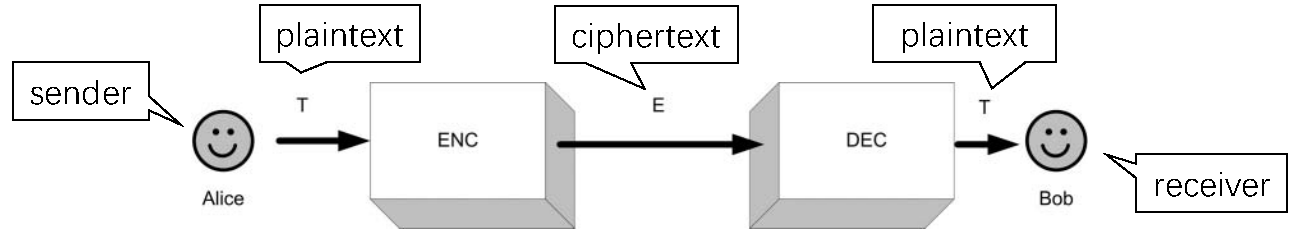
\includegraphics[width=\textwidth]{cryptography-model}
	\caption{The standard cryptography model.}
	\label{fig:cryptography model}
\end{figure}
	
The whole procedure can be divided into two parts:
\begin{itemize}
	\item Encoder (ENC) is responsible for encoding the input plaintext into ciphertext, which can be formulated as $\textrm{ENC}(T,K_{E})=E$ where $T$ is the plaintext, $K_E$ is encryption key, and $E$ is the ciphertext.
	
	\item Decoder (DEC) is responsible for decoding the received ciphertext into plaintext, which can be formulated as $\textrm{DEC}(E, K_D)=T$ where $K_D$ is the decryption key.
\end{itemize}
$\textrm{DEC}(\textrm{ENC}(T, K_E), K_D)=T$ means that as long as we use the right keys, we can always retrieve the original message intact without any loss of information.

\section{Classic Cryptography}
\subsection{Caesar cipher}
In cryptography, a Caesar cipher\footnote{\url{https://en.wikipedia.org/wiki/Caesar_cipher}} (Figure \ref{subfig:caesar-cipher}), also known as Caesar's cipher, the shift cipher, Caesar's code or Caesar shift, is one of the simplest and most widely known encryption techniques. It is a type of substitution cipher in which each letter in the plaintext is replaced by a letter some fixed number of positions down the alphabet. As shown in Figure \ref{subfig:left-shift-3}, with a left shift of 3, D would be replaced by A, E would become B, and so on. The method is named after Julius Caesar, who used it in his private correspondence.

The essence of Caesar cipher is a simple linear mapping, which has high statistical correlation between the letter in plaintext and that in the ciphertext. This means that by graphing the frequencies of letters in the ciphertext, and by knowing the expected distribution of those letters in the original language of the plaintext, a human can easily spot the value of the shift by looking at the displacement of particular features of the graph. This is known as frequency analysis. As shown in Figure \ref{subfig:letter-distribution}, in the English language the plaintext frequencies of the letters E, T, (usually most frequent), and Q, Z (typically least frequent) are particularly distinctive.

\begin{figure}[h]
	\centering
	\subfloat[Caesar cipher]
	{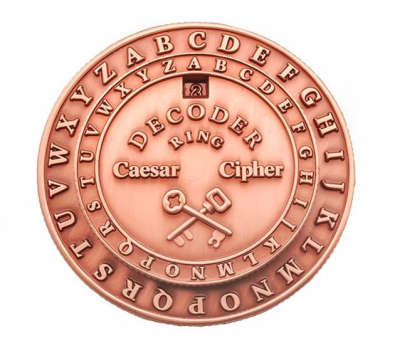
\includegraphics[width=0.25\textwidth]{caesar-cipher}
		\label{subfig:caesar-cipher}}
	\hspace{0.1\textwidth}
	\subfloat[A mapping example of left shift of three]
	{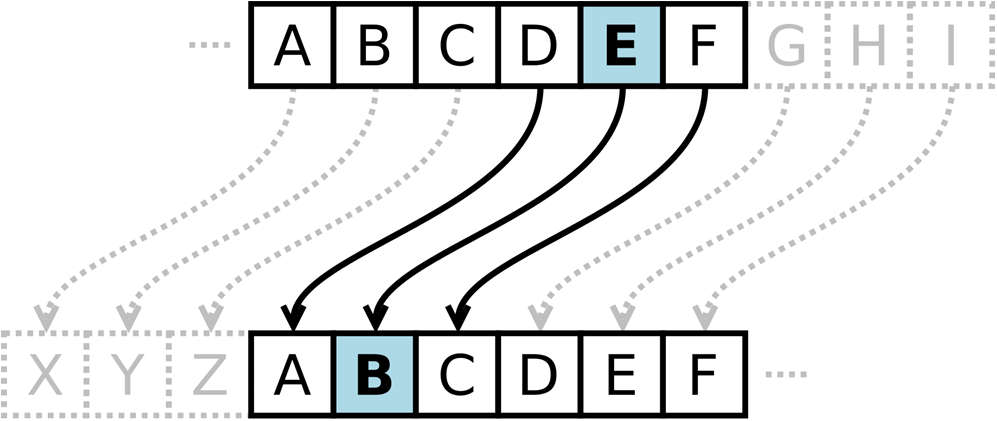
\includegraphics[width=0.55\textwidth]{left-shift-3}
		\label{subfig:left-shift-3}}\\
	\subfloat[Letter distribution in English]
	{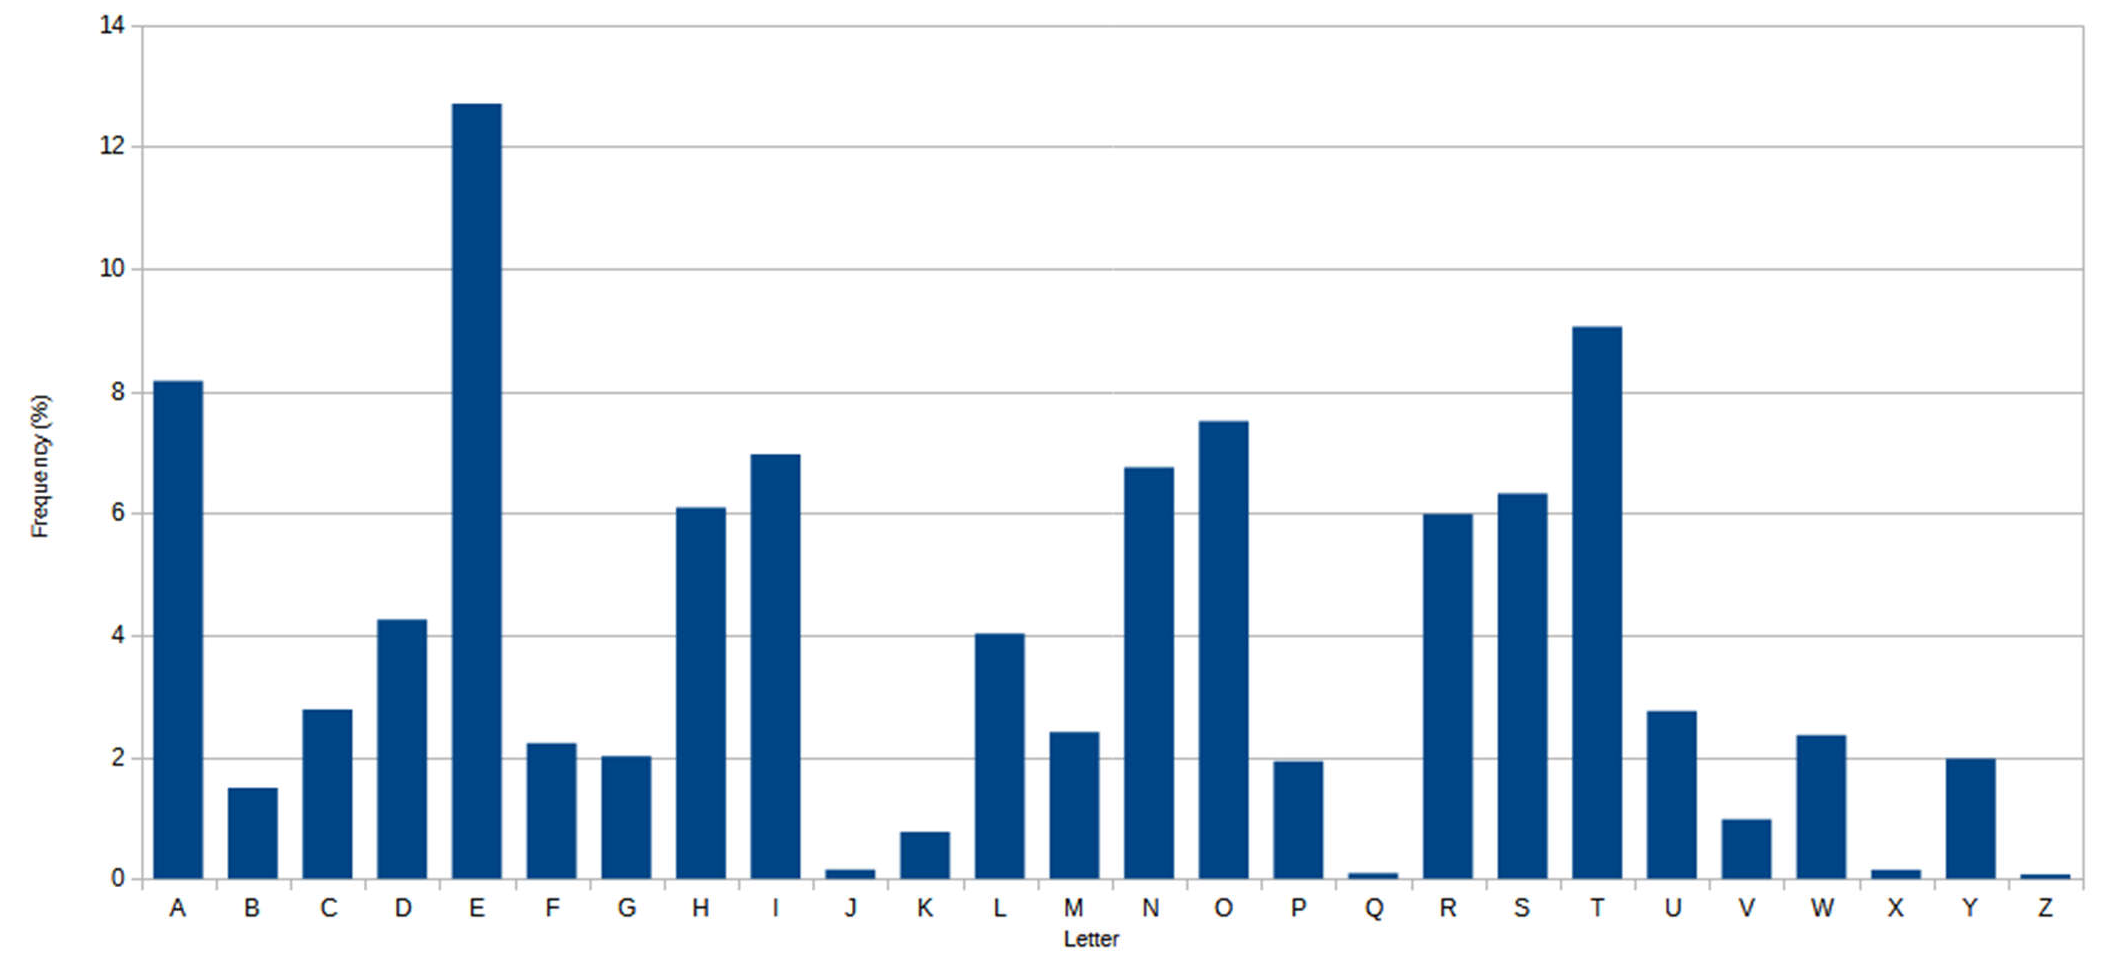
\includegraphics[width=\textwidth]{letter-distribution}
		\label{subfig:letter-distribution}}
	\caption{Caesar cipher's device, scheme, and defect.}
	\label{fig:caesar-cipher}
\end{figure}

\subsection{One-Time-Pad protocol}
In cryptography, the one-time-pad (OTP) protocol\footnote{\url{https://en.wikipedia.org/wiki/One-time_pad}} is an encryption technique that cannot be cracked, but requires the use of a single-use pre-shared key that is not smaller than the message being sent. In this technique, a plaintext is paired with a random secret key (also referred to as a one-time pad). Then, each bit or character of the plaintext is encrypted by combining it with the corresponding bit or character from the pad using modular addition.

\begin{figure}[h]
	\centering
	\includegraphics[width=0.6\textwidth]{otp}
	\caption{The one-time-pad protocol.}
	\label{fig:otp}
\end{figure}

In OTP protocol, both encryption and decryption end share the same key $K$ in the communication process, which means $K_E=K_D=K$. As shown in Figure \ref{fig:otp}, assume that both encoder and decoder share the same working function $\textrm{ENC}(T,K)=\textrm{DEC}(T,K)=T\oplus K$, than the receiver can decode the ciphertext and get the original message as follows 
\begin{equation}
	\begin{aligned}
		\textrm{DEC}(\textrm{ENC}(T,K_E),K_D)&=\textrm{DEC}(T\oplus K, K)\\
		&=(T\oplus K)\oplus K\\
		&=T\oplus (K\oplus K)\\
		&=T		
	\end{aligned}
\end{equation}

The merit of OTP protocol is that it cannot be cracked, but meanwhile, it has two obvious drawbacks. First, the key in OTP must be longer than the message being sent, which is extremely inconvenient in the transmission and storage process; Second, the key cannot be re-used because of the risk of information leakage\footnote{The eavesdropper may infer part of the original message from the multiple intercepted ciphertext if the key is reused because $E_1\oplus E_2=(T_1\oplus K)\oplus (T_2\oplus K)=T_1\oplus K\oplus K\oplus T_2=T_1\oplus T_2$}. 

\subsection{Diffie-Hellman key exchange}
To eliminate risks in the key distribution process, Whitfield Diffie and Martin Hellman devised the Diffie-Hellman key exchange method to securely exchange cryptographic keys over a public channel.  

\begin{figure}[h]
	\centering
	\subfloat[An illustration example]
	{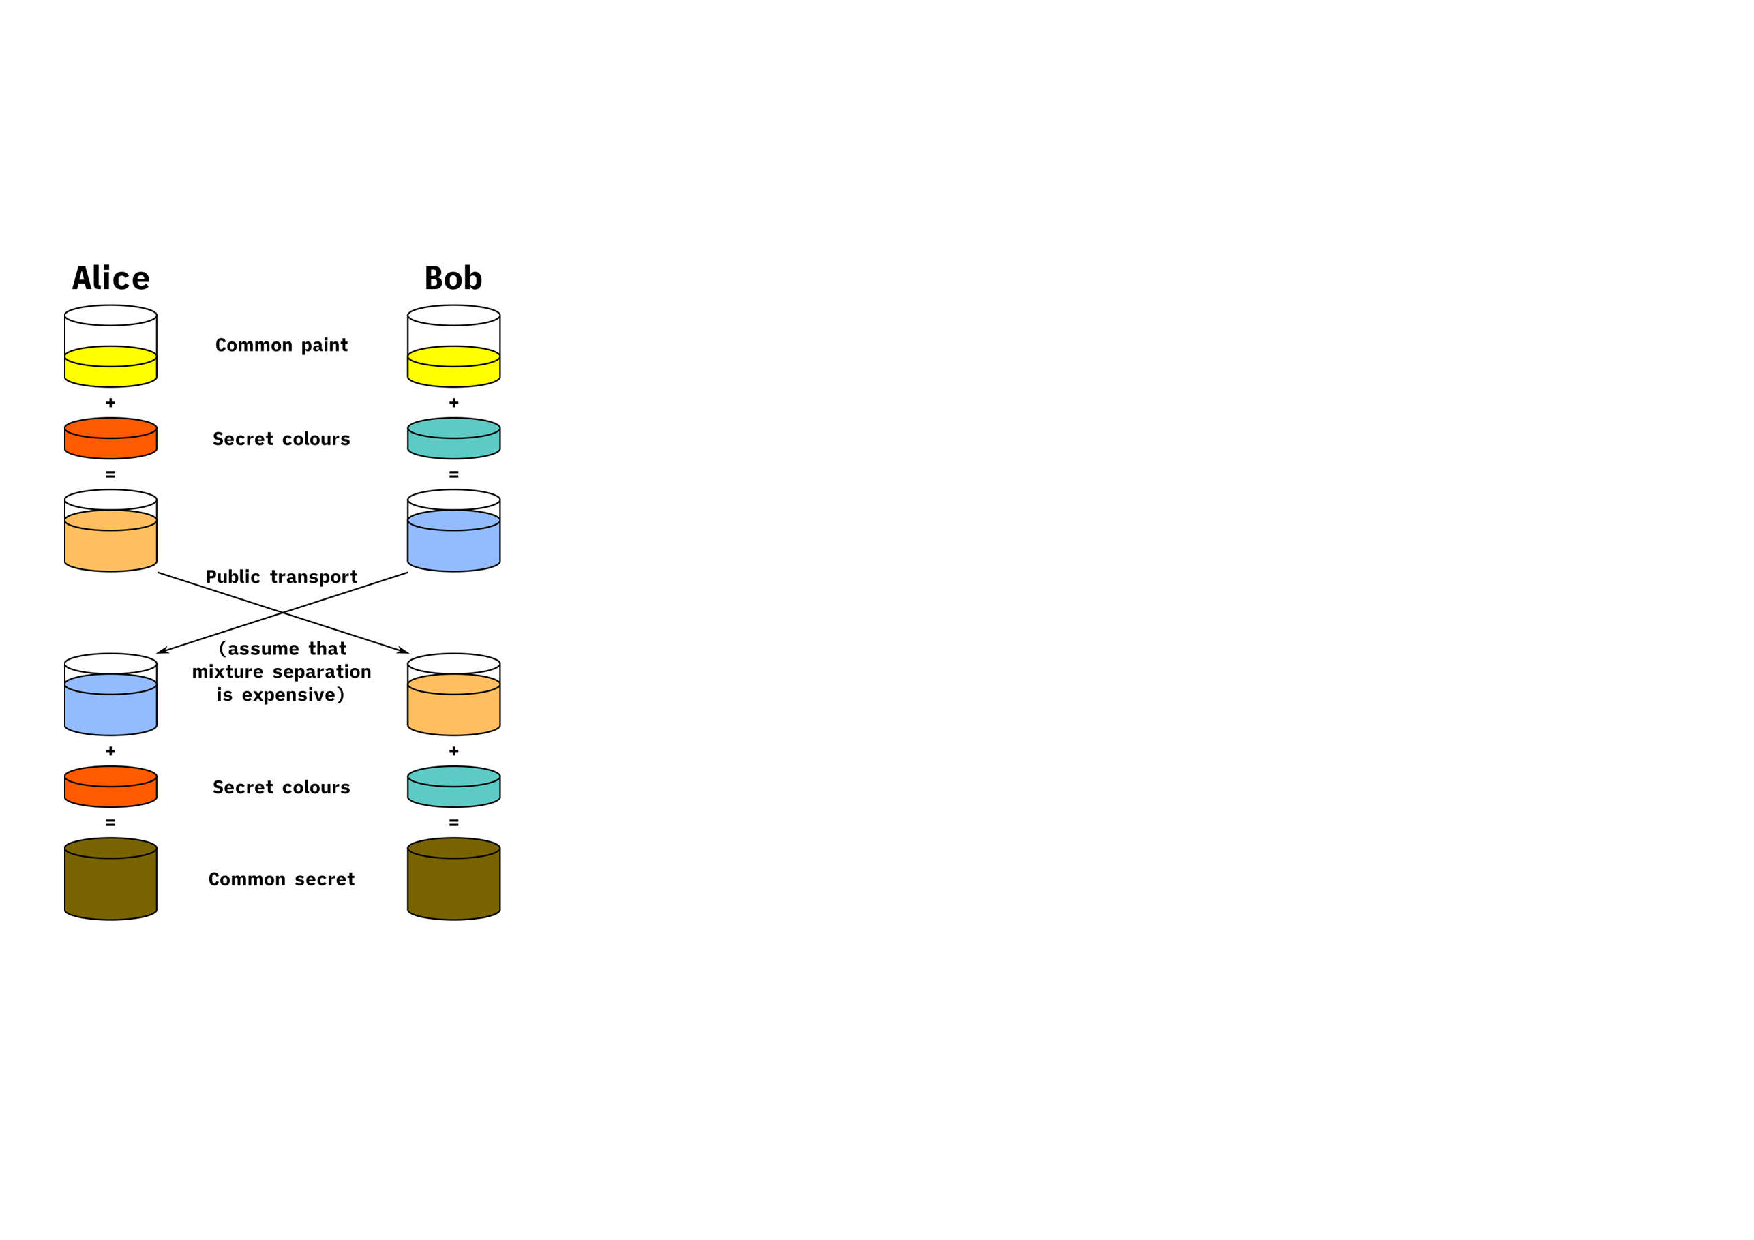
\includegraphics[width=0.25\textwidth]{DH-color}
		\label{subfig:DH-color}}
	\hspace{0.05\textwidth}
	\subfloat[A numerical example]
	{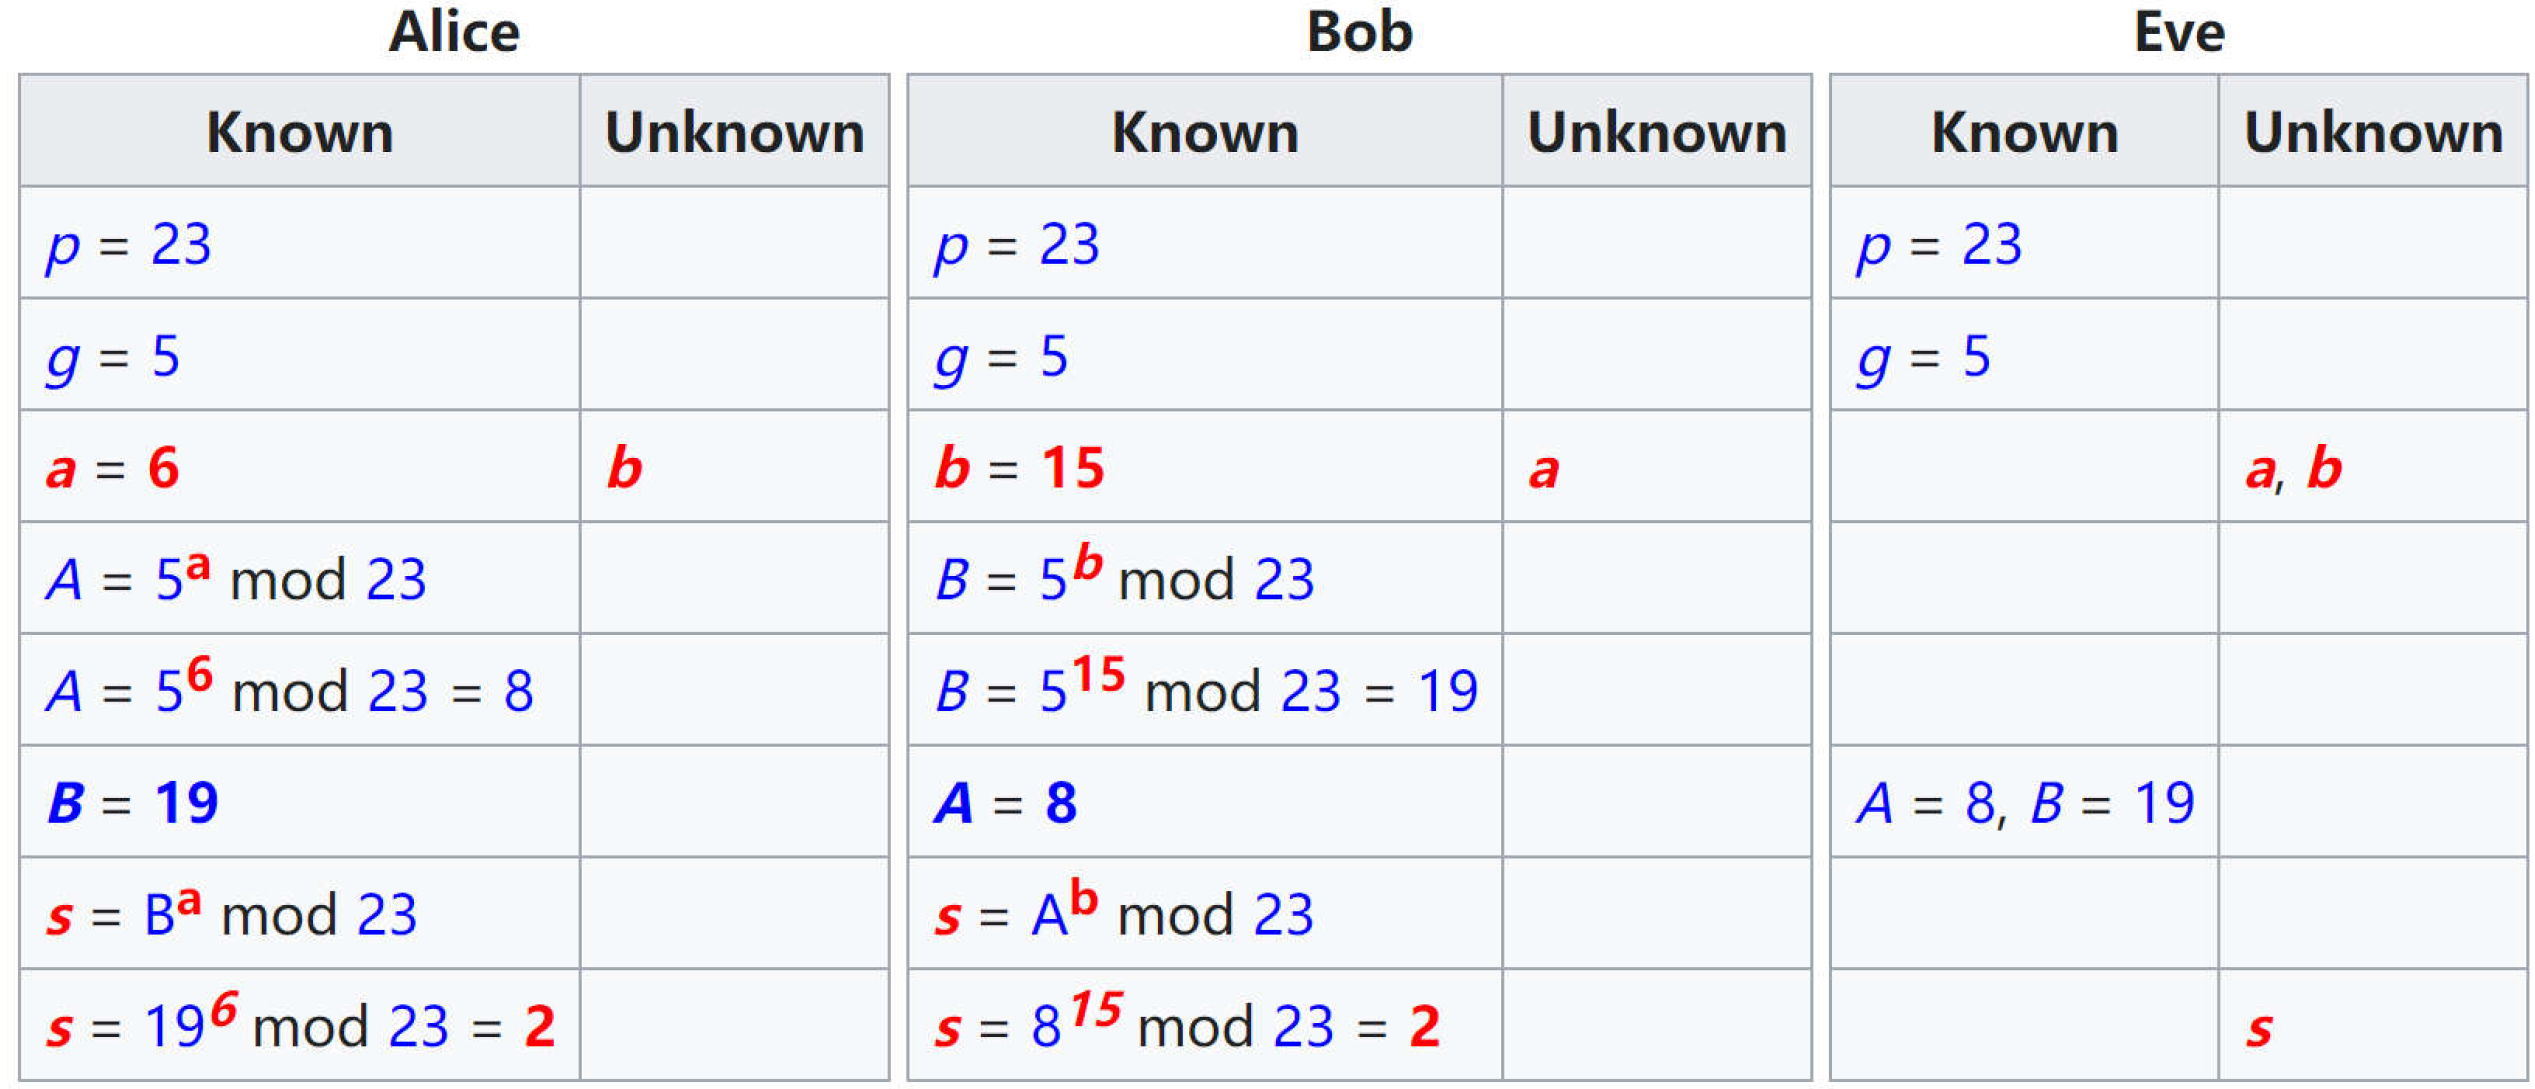
\includegraphics[width=0.6\textwidth]{DH-example}
		\label{subfig:DH-example}}
	\caption{Illustrative and numerical examples of Diffie-Hellman key exchange.}
	\label{fig:DH}
\end{figure}

An analogy illustrates the concept of public key exchange by using colors instead of very large numbers. As shown in Figure \ref{subfig:DH-color}, the Diffie-Hellman key exchange process begins by having the two parties, Alice and Bob, publicly agree on an arbitrary starting color that does not need to be kept secret. In this example, the color is yellow. Each person also selects a secret color that they keep to themselves – in this case, red and cyan. The crucial part of the process is that Alice and Bob each mix their own secret color together with their mutually shared color, resulting in orange-tan and light-blue mixtures respectively, and then publicly exchange the two mixed colors. Finally, each of them mixes the color they received from the partner with their own private color. The result is a final color mixture (yellow-brown in this case) that is identical to their partner's final color mixture.

The numerical example of the above colorization process is shown in Figure  \ref{subfig:DH-example}. The pigment mixing process is formulated as a classic trapdoor function, also dubbed as one-way function, \textit{i.e.,} modular exponentiation $f(x)=g^x mod p$. The forward computation, from $x$ to $f(x)$, is easy and fast, while the backward computation, from $f(x)$ to $x$, is extremely hard and computationally prohibitive. In the table, $a$ and $b$ represent the secret color that Alice and Bob keep to themselves at the beginning, $A$ and $B$ represent the publicly exchanged color, and $s$ is the final shared color mixture. Thanks to the one-way property of the modular exponentiation, even Eve got $A$ and $B$, he cannot recover $a$ and $b$, not to mention the exchanged key $s$.

\subsection{Public- and private-key cryptography}
According to the availability of the encryption key, cryptography algorithm can be divided into private-key cryptography and public-key cryptography (Figure \ref{fig:public-private-key-cryptography}).

\begin{figure}[h]
	\centering
	\subfloat[private-key cryptography]
	{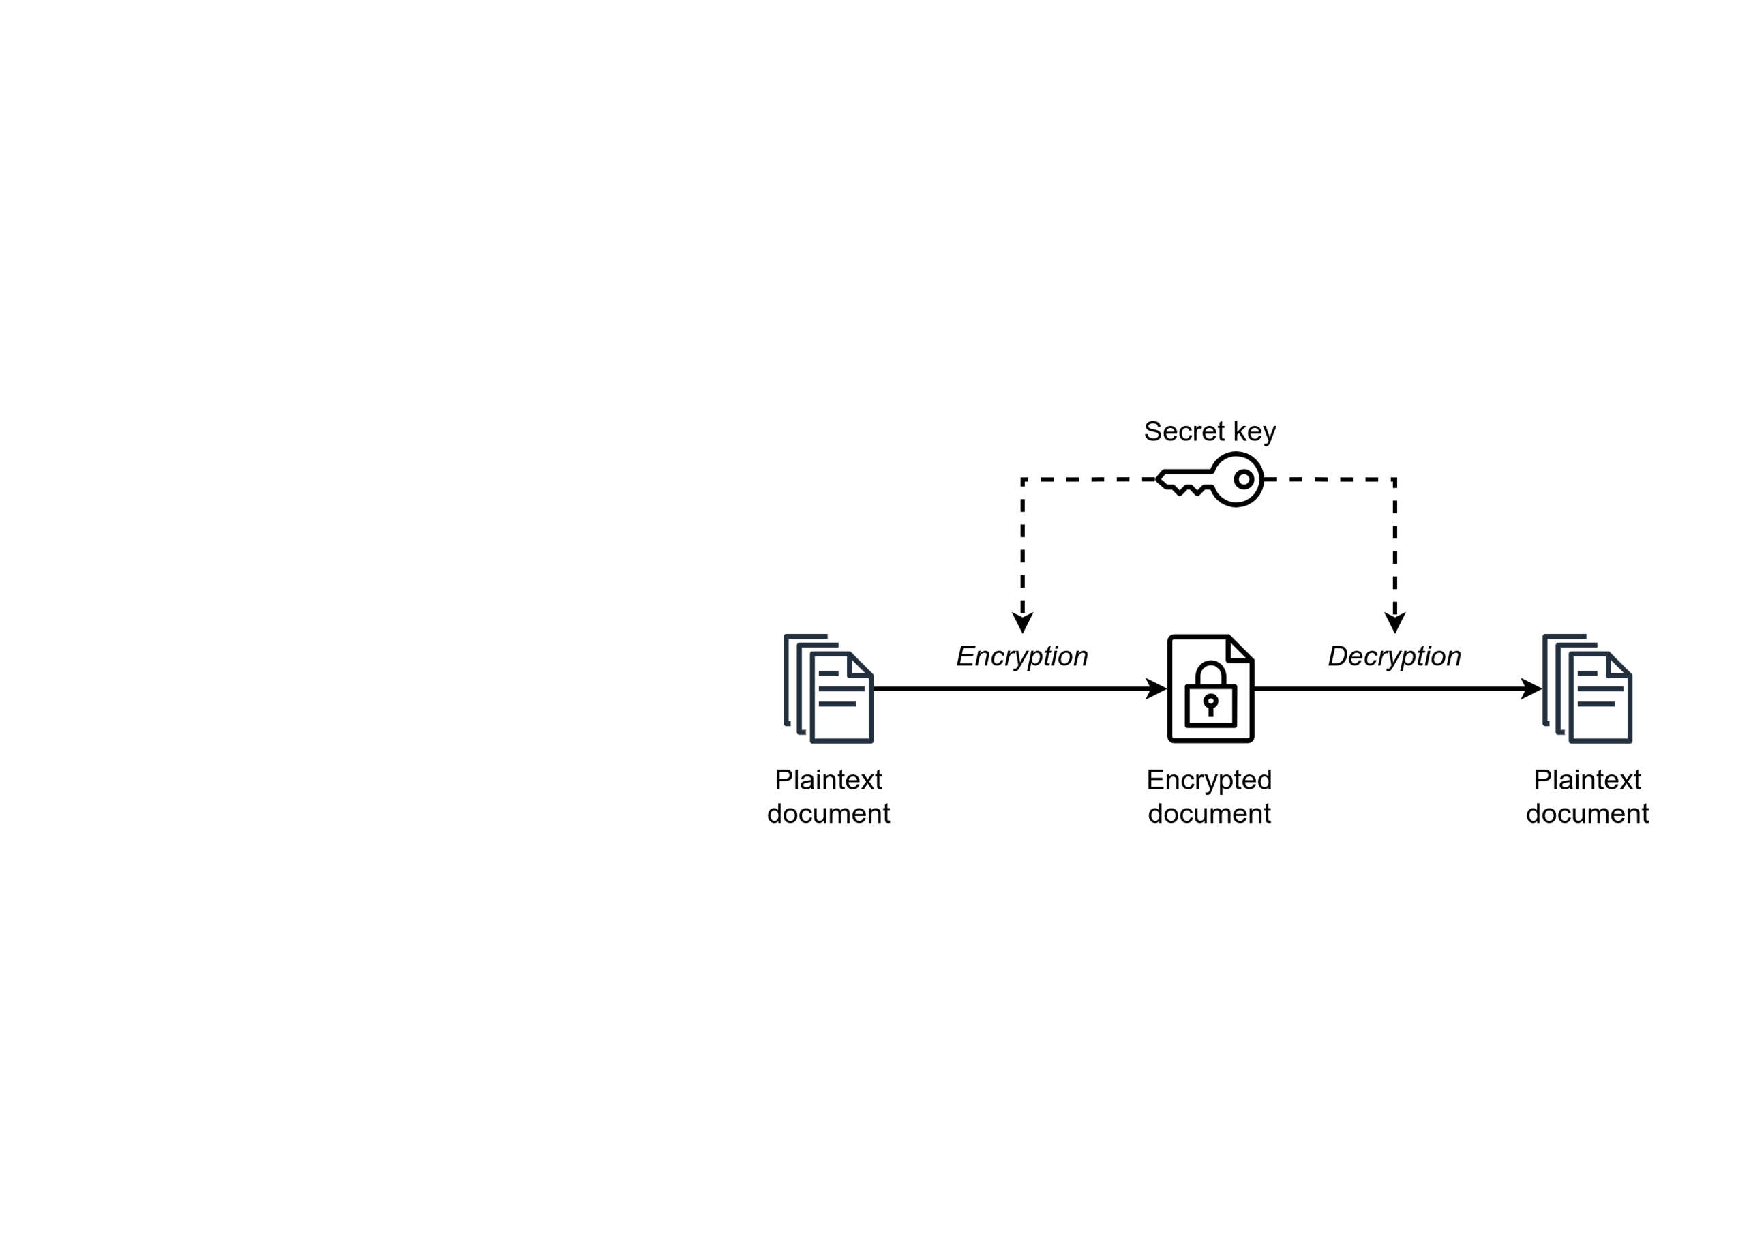
\includegraphics[width=0.5\textwidth]{private-key-cryptography}
		\label{subfig:private-key-cryptography}}
	\hspace{0.05\textwidth}
	\subfloat[public-key cryptography]
	{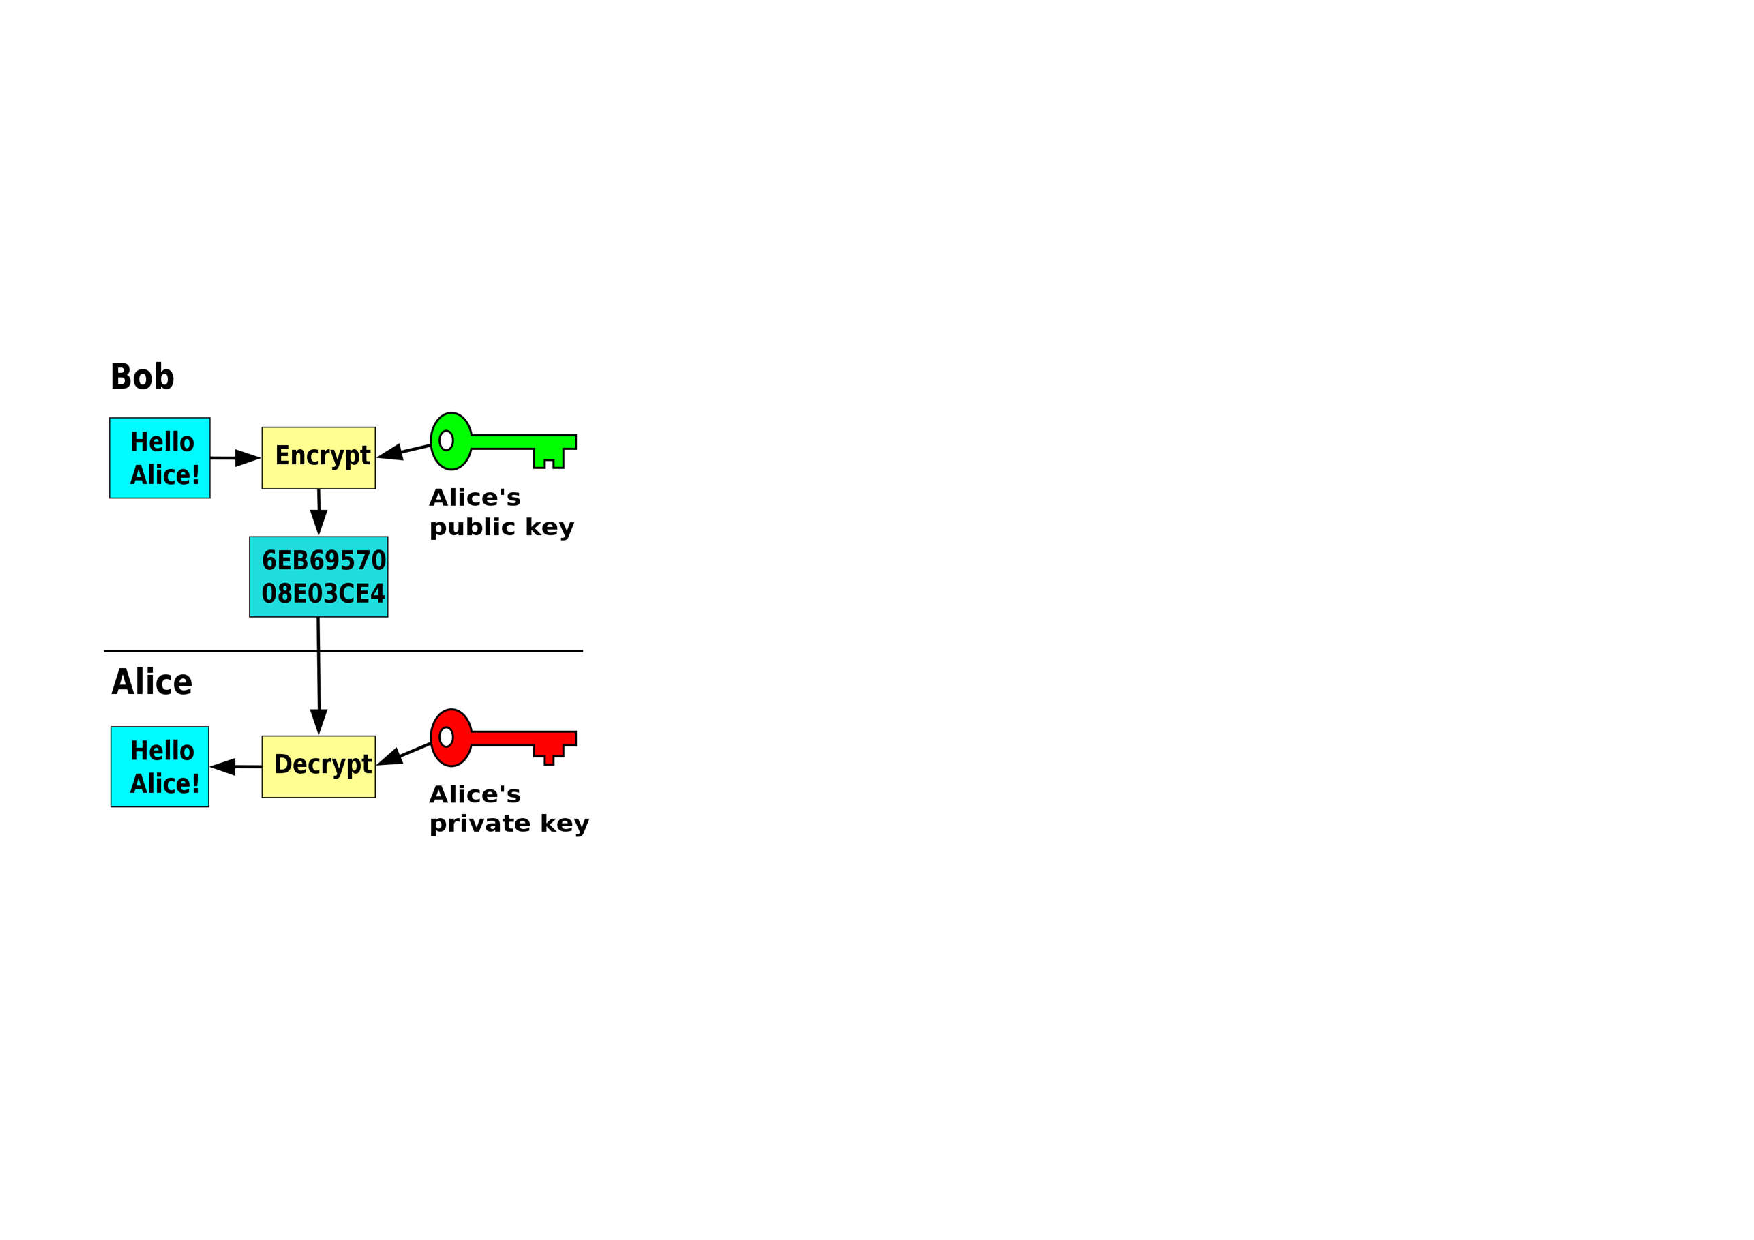
\includegraphics[width=0.4\textwidth]{public-key-cryptography}
		\label{subfig:public-key-cryptography}}
	\caption{Diagrams of private-key cryptography and public-key cryptography.}
	\label{fig:public-private-key-cryptography}
\end{figure}

\textbf{private-key cryptography}, or symmetric cryptography, uses the same cryptographic keys for both the encryption of plaintext and the decryption of ciphertext. The keys, in practice, represent a shared secret between two or more parties that can be used to maintain a private information link (Figure \ref{subfig:private-key-cryptography}). The requirement that both parties have access to the secret key is one of the main drawbacks of symmetric-key encryption, in comparison to public-key encryption. OTP protocal is a typical private-key algorithm.

\textbf{Public-key cryptography}, or asymmetric cryptography, is the field of cryptographic systems that use pairs of related keys. Each key pair consists of a public key and a corresponding private key. Key pairs are generated with cryptographic algorithms based on mathematical problems termed one-way functions. In a public-key encryption system, anyone with a public key can encrypt a message, yielding a ciphertext, but only those who know the corresponding private key can decrypt the ciphertext to obtain the original message (Figure \ref{subfig:public-key-cryptography}). Diffie-Hellman key exchange belongs to the public-key cryptography.

The plus side of public-key cryptography is that it does have key distribution problem. In contrast, the minus sides include: (1) the one-way property of trapdoor function is a temporary fact that may disappear in the future; (2) public-key cryptography is usually slower than private-key cryptography.

Typical issues in classic cryptography include: (1) success communication; (2) intrusion detection, \textit{i.e.}, Alice and Bob would like to determine whether Eve is, in fact, eavesdropping; (3) authentication, \textit{i.e.}, we would like to ensure that nobody is impersonating Alice and sending false messages.


\section{Quantum Key Exchange}
Due to the peculiar effect of quantum observation and measurement, eavesdropping in the classical world has a very different manifestation from that in the quantum world. Specifically, in the classic world, Eve can make copies of arbitrary portions of the encrypted bit stream, and he can listen without affecting the bit stream. While in the quantum world, Eve cannot make perfect copies of the qubit stream because of the no-cloning theorem, and the very act of measuring the qubit stream alters it. 

\subsection{The BB84 protocol}
The first quantum key exchange protocol was introduced by Charles Bennett
and Gilles Brassard in 1984, and hence the name BB84. 

\textbf{Problem setting.} Alice’s goal is to send Bob a key via a quantum channel. Just as in the One-TimePad protocol, her key is a sequence of random (classical) bits obtained, perhaps, by tossing a coin. Alice will send a qubit each time she generates a new bit of her key. But which qubit should she send?

\textbf{Plus and times bases.} In this protocol, Alice will employ two different orthogonal bases shown in Figure \ref{fig:plus-times-basis}. The left part shows the ``plus'' basis whose formulation is 
\begin{equation}
	+ = \{\ket{\rightarrow},\ket{\uparrow}\}=\big{\{}[1,0]^{\top},[0,1]^{\top}\big{\}}
\end{equation}
and the right part shows the ``times'' basis whose formulation is
\begin{equation}
	\times = \{\ket{\nwarrow},\ket{\nearrow}\}=\Big{\{}\frac{1}{\sqrt{2}}[-1,1]^{\top},\frac{1}{\sqrt{2}}[1,1]^{\top}\Big{\}}
\end{equation}

\begin{figure}[h]
	\centering
	\subfloat[The plus basis]
	{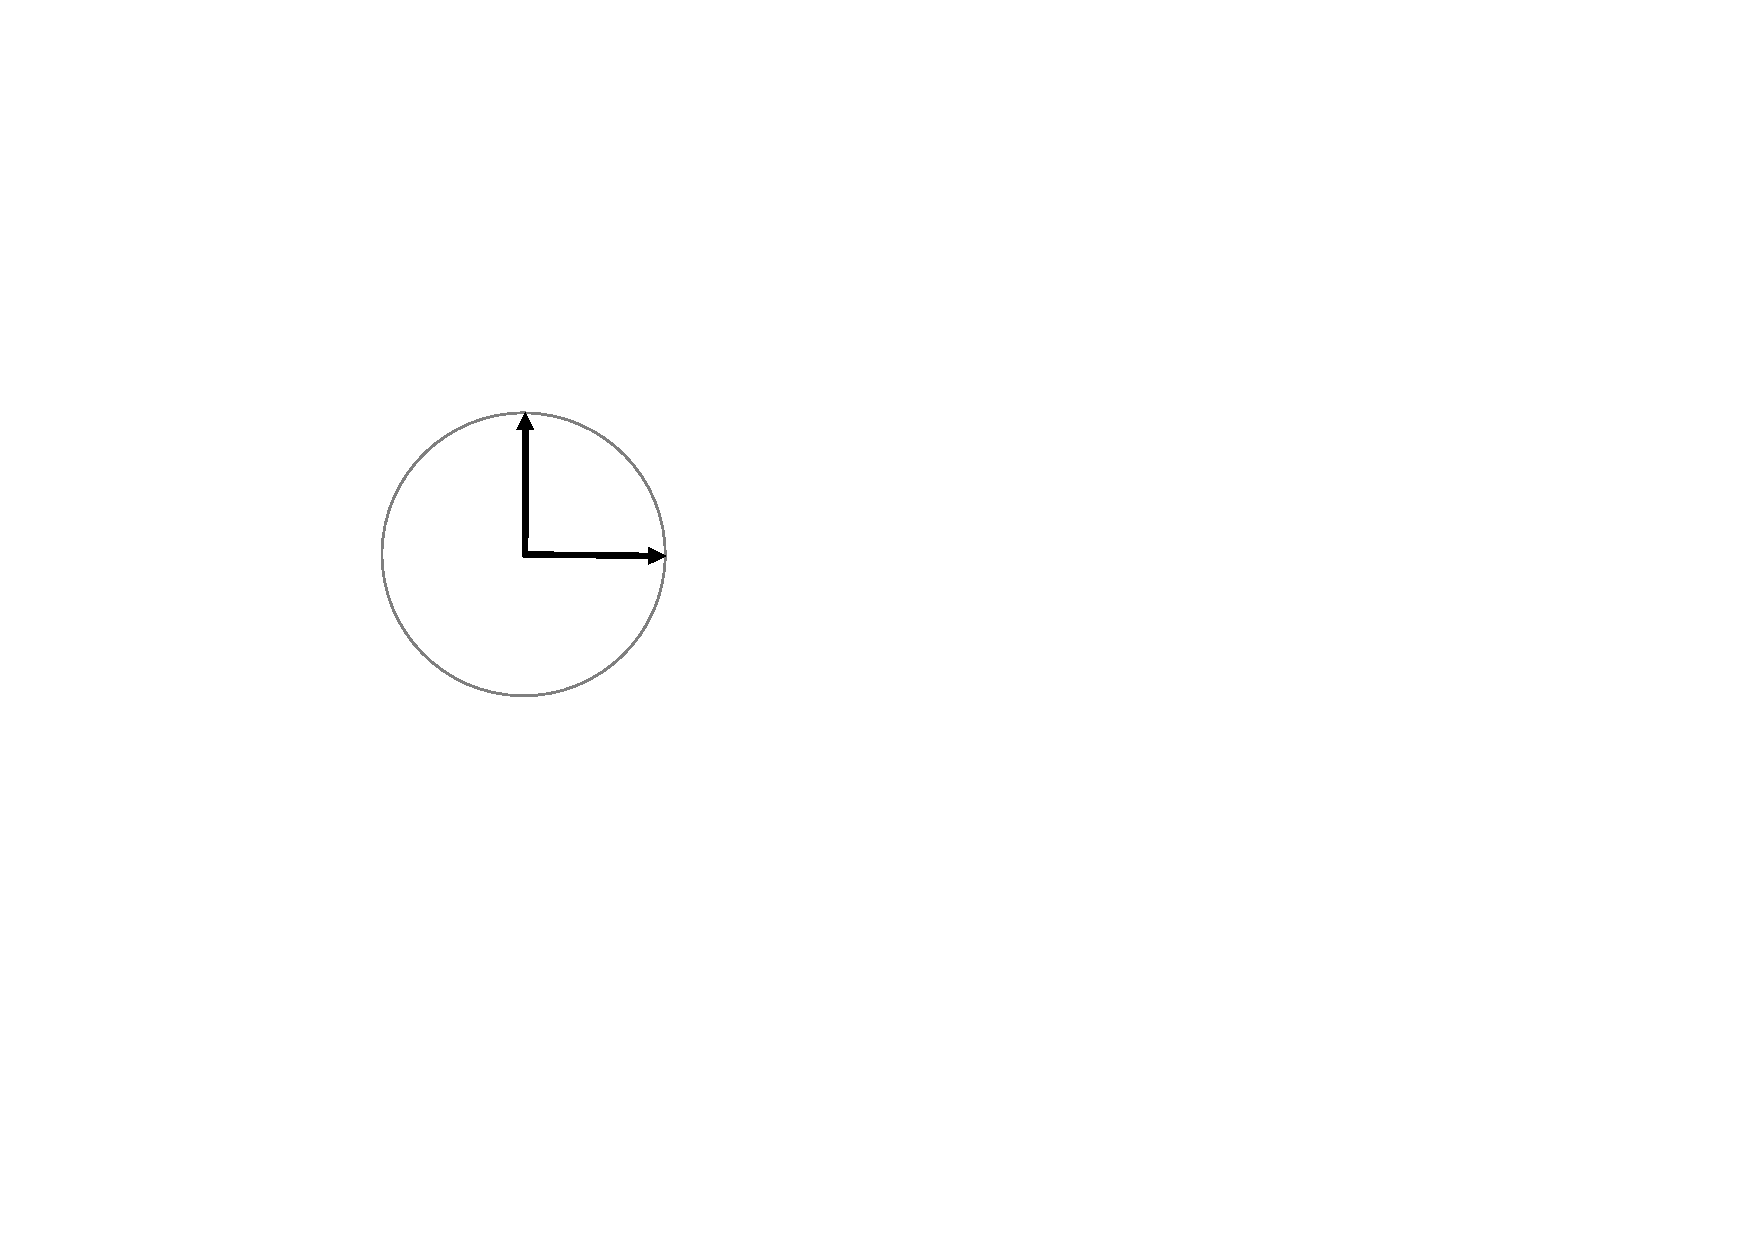
\includegraphics[width=0.3\textwidth]{plus-basis}
		\label{subfig:plus-basis}}
	\hspace{0.2\textwidth}
	\subfloat[The times basis]
	{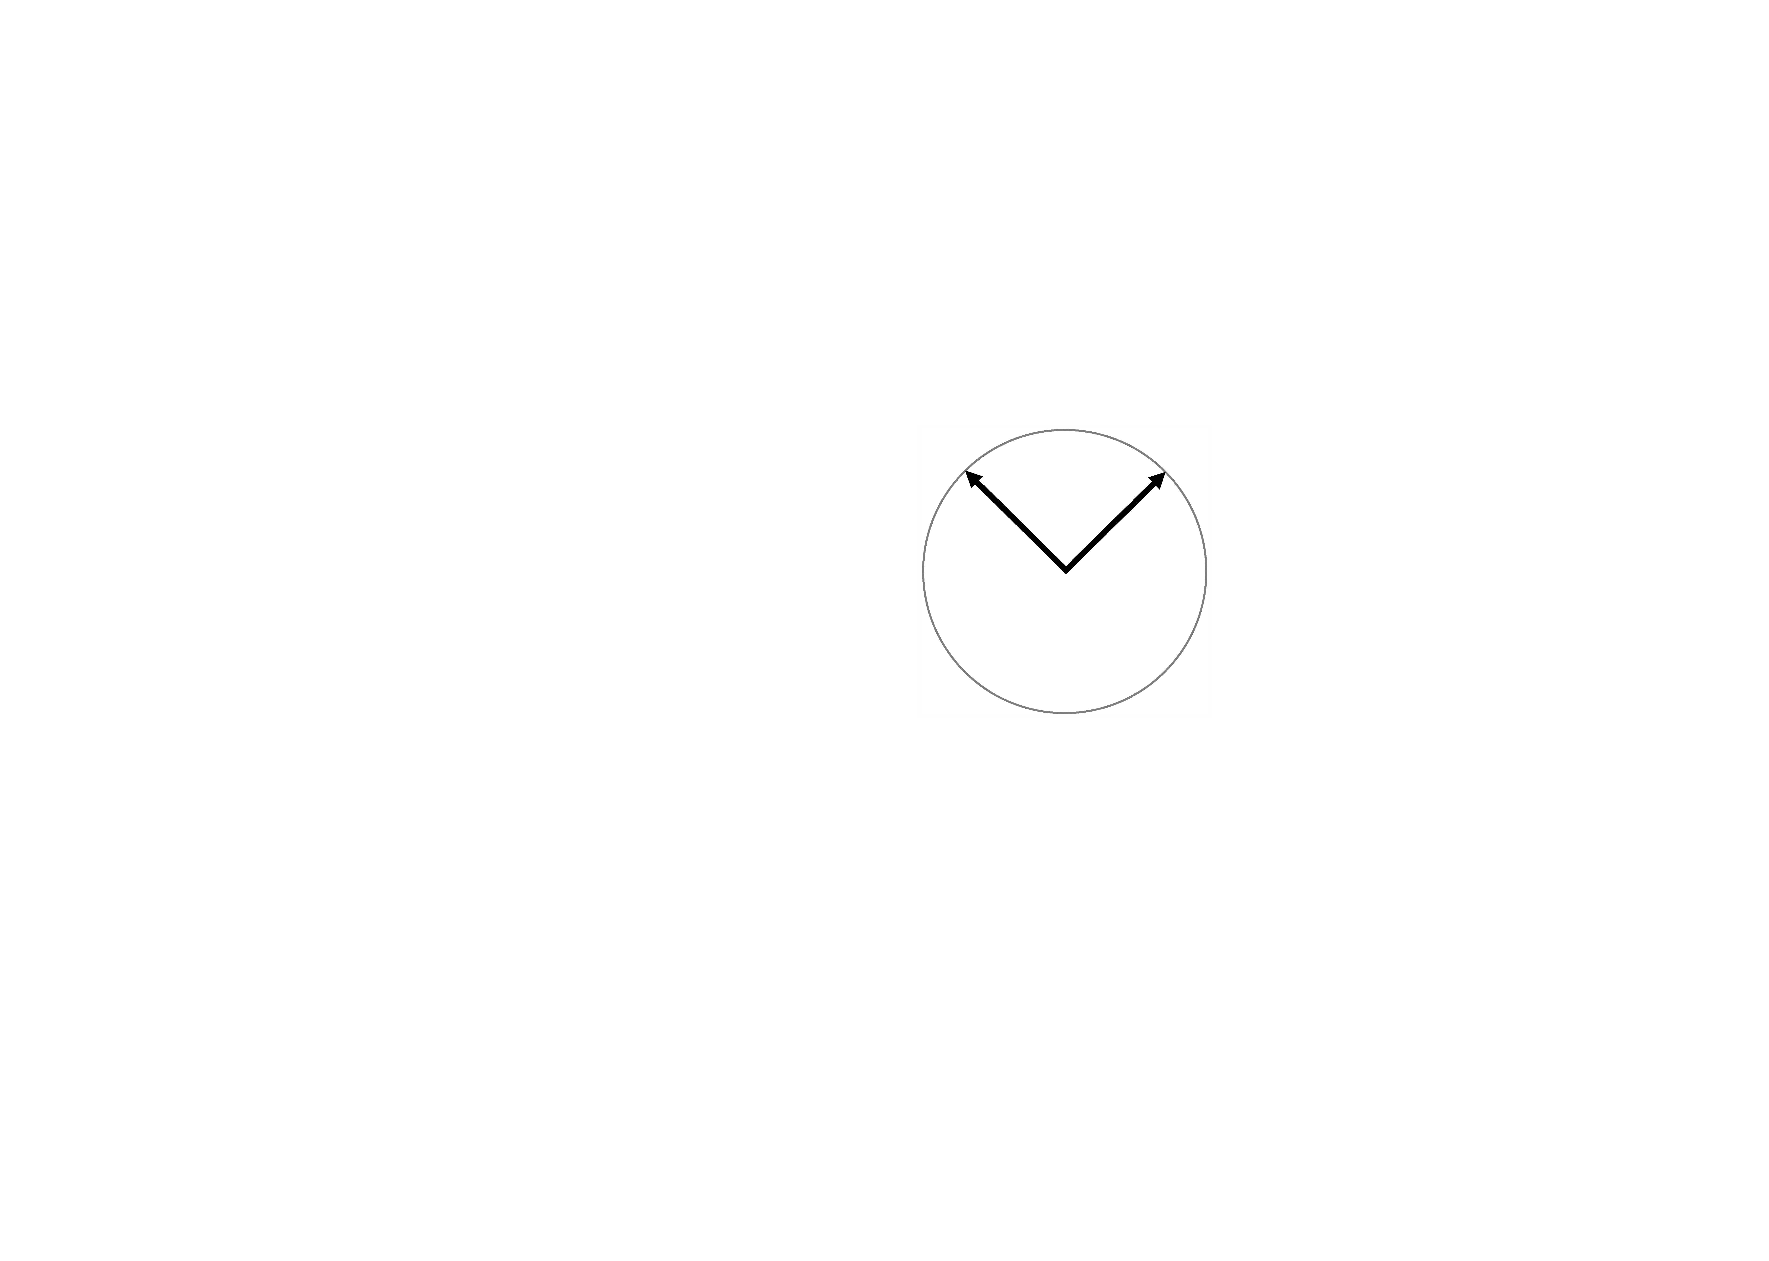
\includegraphics[width=0.3\textwidth]{times-basis}
		\label{subfig:times-basis}}
	\caption{Two basis used in BB84.}
	\label{fig:plus-times-basis}
\end{figure}

\textbf{Cross representation.} The base vector in one basis can be linearly represented by base vectors in another basis:
\begin{itemize}
	\item $\ket{\nwarrow}$ with respect to $+$ will be $\frac{1}{\sqrt{2}}\ket{\uparrow}-\frac{1}{\sqrt{2}}\ket{\rightarrow}$.
	
	\item $\ket{\nearrow}$ with respect to $+$ will be $\frac{1}{\sqrt{2}}\ket{\uparrow}+\frac{1}{\sqrt{2}}\ket{\rightarrow}$.
	
	\item $\ket{\uparrow}$ with respect to $\times$ will be $\frac{1}{\sqrt{2}}\ket{\nearrow}+\frac{1}{\sqrt{2}}\ket{\nwarrow}$.
	
	\item $\ket{\rightarrow}$ with respect to $\times$ will be $\frac{1}{\sqrt{2}}\ket{\nearrow}-\frac{1}{\sqrt{2}}\ket{\nwarrow}$.
\end{itemize}

\textbf{Mapping table.} Alice translates her classic key bits into qubits according to a mapping vocabulary shown in the following table.
\begin{table}[h]
	\centering
	%\caption{Mapping table between qubits and classic bits}
	\begin{tabular}{ccc}
		\toprule  
		State/Basis&$+$&$\times$ \\ 
		\midrule
		$\ket{0}$&$\ket{\rightarrow}$&$\ket{\nearrow}$ \\
		$\ket{1}$&$\ket{\uparrow}$&$\ket{\nwarrow}$ \\
		\bottomrule  
	\end{tabular}
\end{table}
For example, in the $+$ basis, a $\ket{\rightarrow}$ will correspond to a $\ket{0}$. If Alice wants to work in the $\times$ basis and wants to convey a $\ket{1}$, she will send a $\ket{\nwarrow}$. Similarly, if Alice sends a $\ket{\uparrow}$ and Bob measures a $\ket{\uparrow}$ in the $+$ basis, he should record a $\ket{1}$.

\textbf{BB84 protocol.} There are totally $4$ steps in the BB84 protocol:
\begin{enumerate}[\textbf{step} 1]
	\item (Alice)
		\begin{itemize}
			\item randomly determine classical bits to send
			\item randomly determine the bases to send bits
			\item send the bits in their appropriate basis
			\begin{figure}[h]
				\centering
				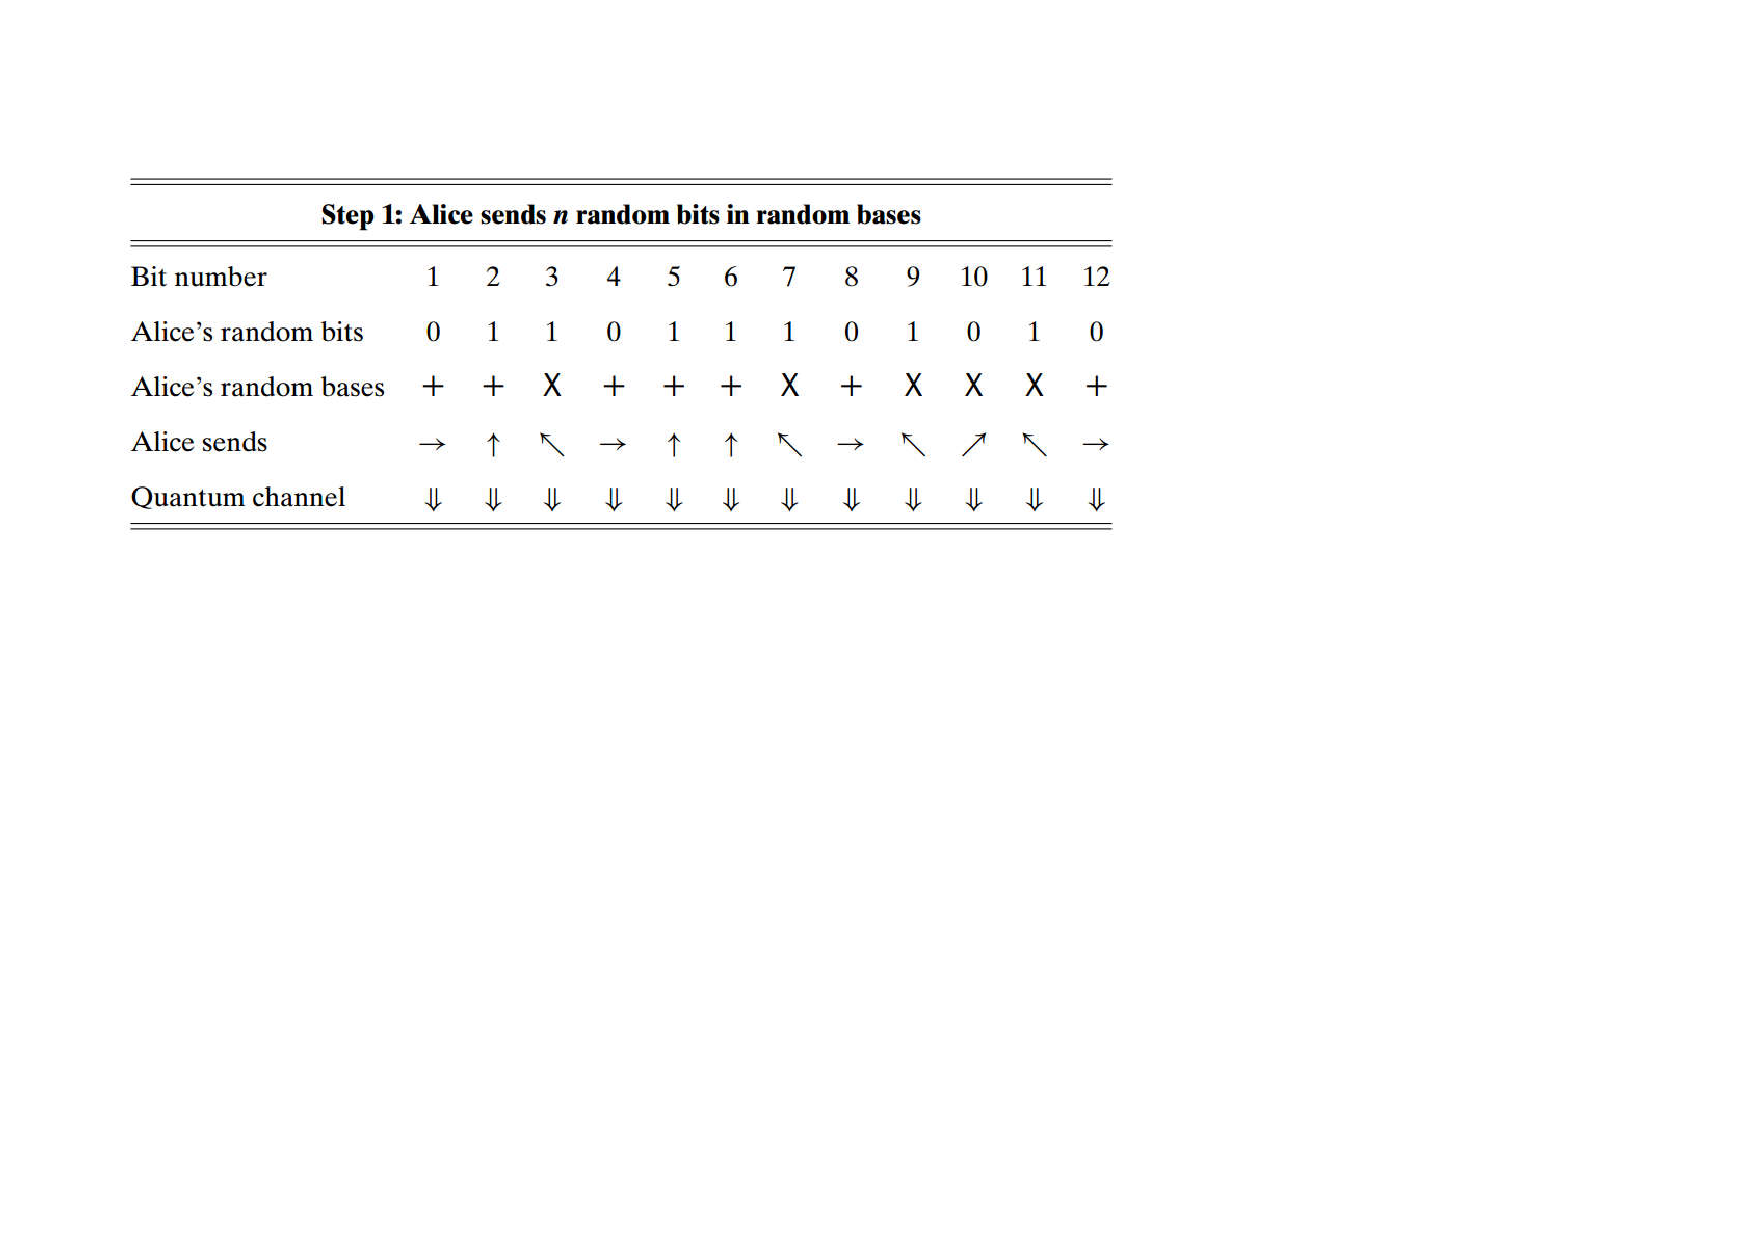
\includegraphics[width=0.8\textwidth]{BB84-step1}
				\label{fig:BB84-step1}
			\end{figure}
		\end{itemize}
	\item (Bob)
		\begin{itemize}
			\item randomly determine the bases to receive bits
			\item measure the qubit in those random bases 
			\begin{figure}[h]
				\centering
				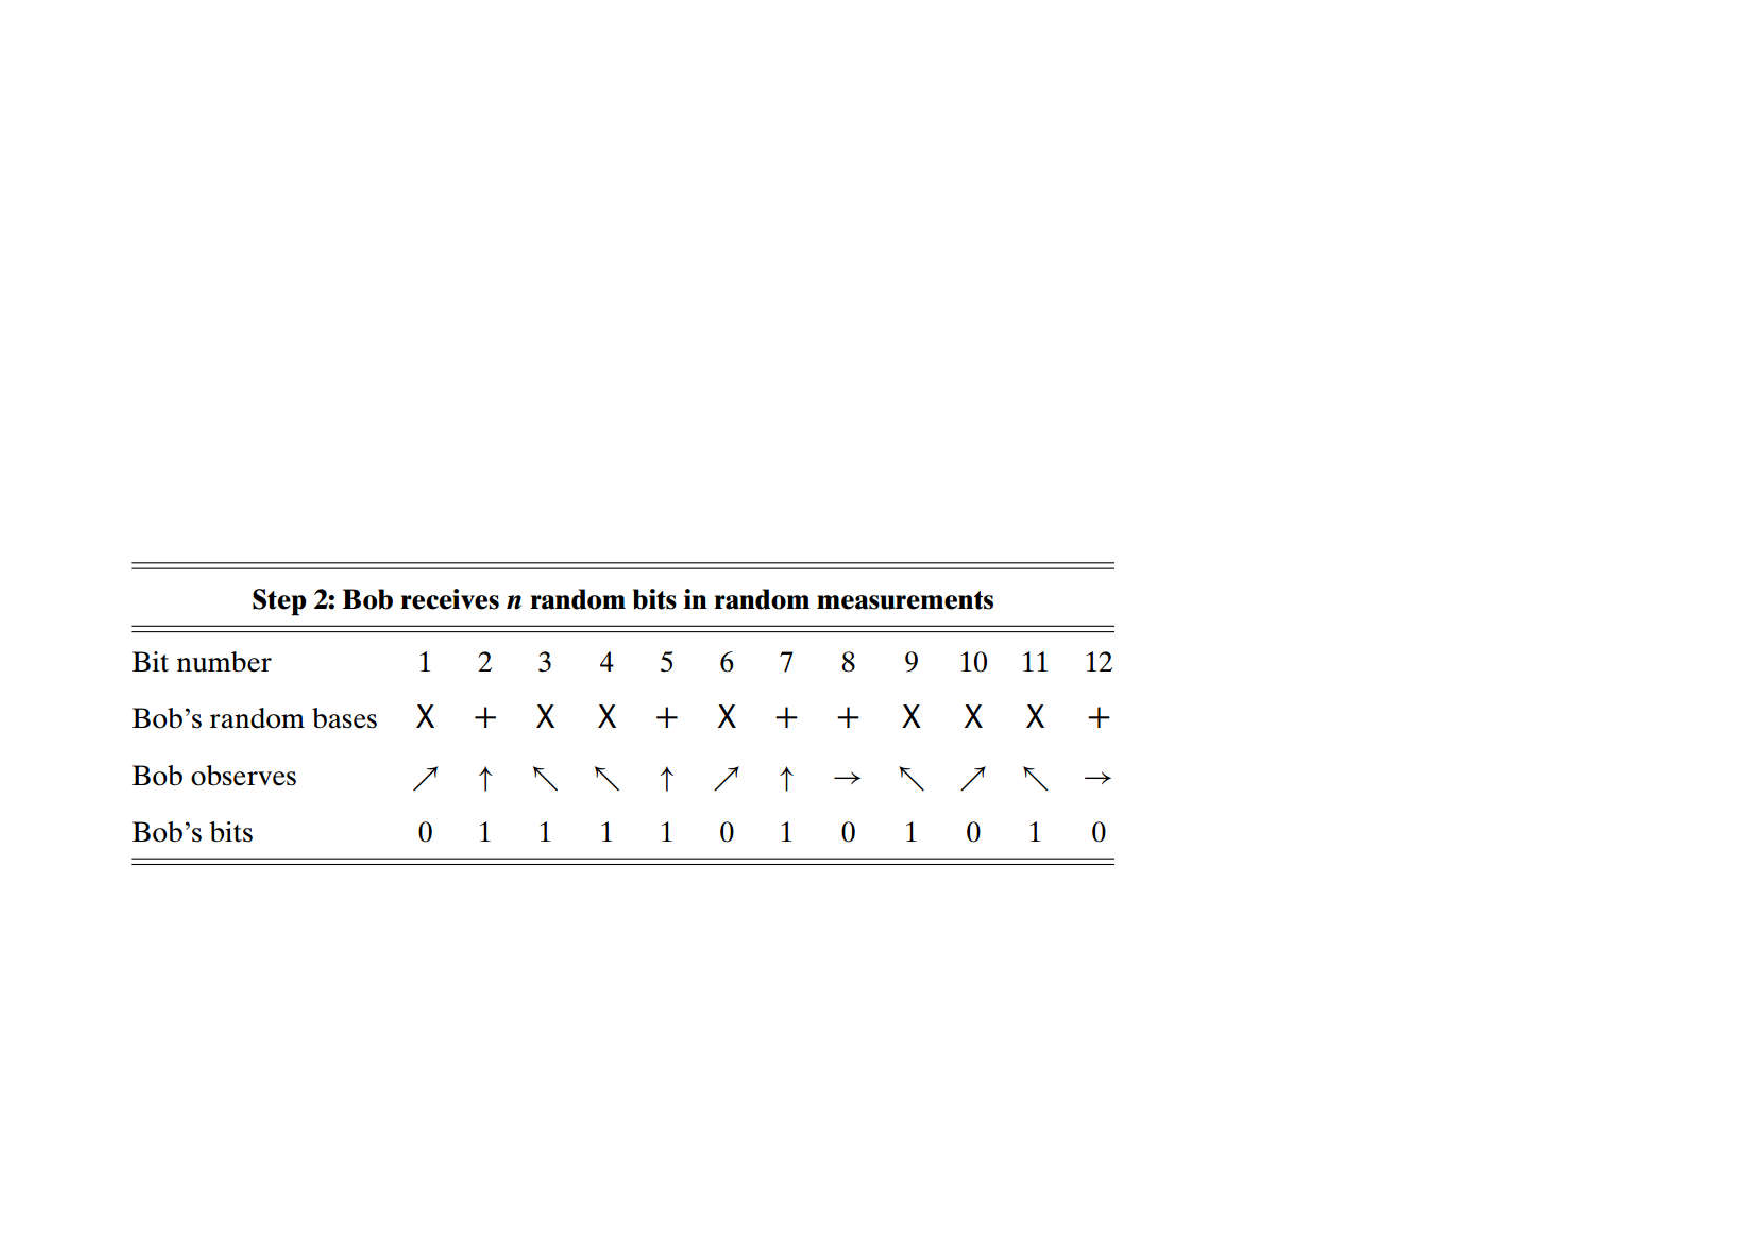
\includegraphics[width=0.8\textwidth]{BB84-step2}
				\label{fig:BB84-step2}
			\end{figure}
		\end{itemize}
		
		When there is no eavesdropping, Bob has $100\%$ probability to get the correct bit with consistent bases, and $50\%$ probability to get the correct bit with inconsistent bases. Hence the expected correct rate (ECR) for Bob getting the correct bit is $\frac{1}{2}\times 1+\frac{1}{2}\times\frac{1}{2}=75\%$.
		
		When there is Eve bugging in, he reads the information that Alice transmits, and meanwhile, sneds that information onward to Bob. In this case, ECR changes into $\frac{3}{4}\times \frac{3}{4}+\frac{1}{4}(\frac{1}{2}\times 0+\frac{1}{2}\times\frac{1}{2})=62.5\%$. The first term means both Eve and Bob get the correct bit, while the second term represents that Eve gets the wrong bit but Bob gets the right one. %So Bob can detect the intrusion by computing the ECR.

	    The following Table gives another solution to calculate the ECR with eavesdropping, where the first stage considers the operations of receiving basis and sending qubit of Eve, and the second stage considers the receiving basis and bit of Bob.
	    
	    \begin{table}[h]
		\hspace{10mm}
		\label{tab:ECR}
		\renewcommand\arraystretch{1.5}	
		\resizebox{0.9\textwidth}{!}{
		\begin{tabular}{c|c|c|c|c}
			\hline
			\hline
			\multicolumn{2}{c|}{{\textbf{Eve}}} & 
			\multicolumn{2}{|c|}{{\textbf{Bob}}} & 
			\multirow{3}{*}{{\textbf{Probability}}} \\
			\cline{1-4}
			\textbf{Receiving basis} & 
			\textbf{Sending qubit} & 
			\textbf{Receiving basis} & 
			\textbf{Receiving bit}  &
			\\
			
			\textbf{(consistent to Alice)} & 
			\textbf{(consistent to Alice)} & 
			\textbf{(consistent to Eve)} & 
			\textbf{(consistent to Alice)} & 
			\\
			\hline
			\hline
			\multirow{2}{*}{$P(\checkmark) = 1/2$} & 
			\multirow{2}{*}{$P(\checkmark) = 1$} & 
			$P(\checkmark) = 1/2$ & 
			$P(\checkmark) = 1$ & 
			\multirow{2}{*}{\Large$\frac{1}{2}\cdot 1\cdot\Big[\frac{1}{2}\cdot1+\frac{1}{2}\cdot\frac{1}{2}\Big]=\frac{6}{16}$} \\
			\cline{3-4}
			&&
			$P(\times) = 1/2$ & 
			$P(\checkmark) = 1/2$ & 
			\\
			
			\hline
			\multirow{4}{*}{$P(\times) = 1/2$} & 
			\multirow{2}{*}{$P(\checkmark) = 1/2$} & 
			$P(\checkmark) = 1/2$ & 
			$P(\checkmark) = 1$ & 
			\multirow{2}{*}{\Large$\frac{1}{2}\cdot \frac{1}{2}\cdot\Big[\frac{1}{2}\cdot1+\frac{1}{2}\cdot\frac{1}{2}\Big]=\frac{3}{16}$} \\
			\cline{3-4}
			&&
			$P(\times) = 1/2$ & 
			$P(\checkmark) = 1/2$ & 
			\\
			\cline{2-5}
			
			&\multirow{2}{*}{$P(\times) = 1/2$} & 
			$P(\checkmark) = 1/2$ & 
			$P(\checkmark) = 0$ & 
			\multirow{2}{*}{\Large$\frac{1}{2}\cdot \frac{1}{2}\cdot\Big[\frac{1}{2}\cdot0+\frac{1}{2}\cdot\frac{1}{2}\Big]=\frac{1}{16}$} \\
			\cline{3-4}
			&&
			$P(\times) = 1/2$ & 
			$P(\checkmark) = 1/2$ & 
			\\
			\hline
			\hline
	\end{tabular}}
\end{table}
	
		

		
	\item (Alice and Bob)
		\begin{itemize}
			\item publicly compare which basis they used at each step
			\item scratch out corresponding bits under different bases
			\begin{figure}[h]
				\centering
				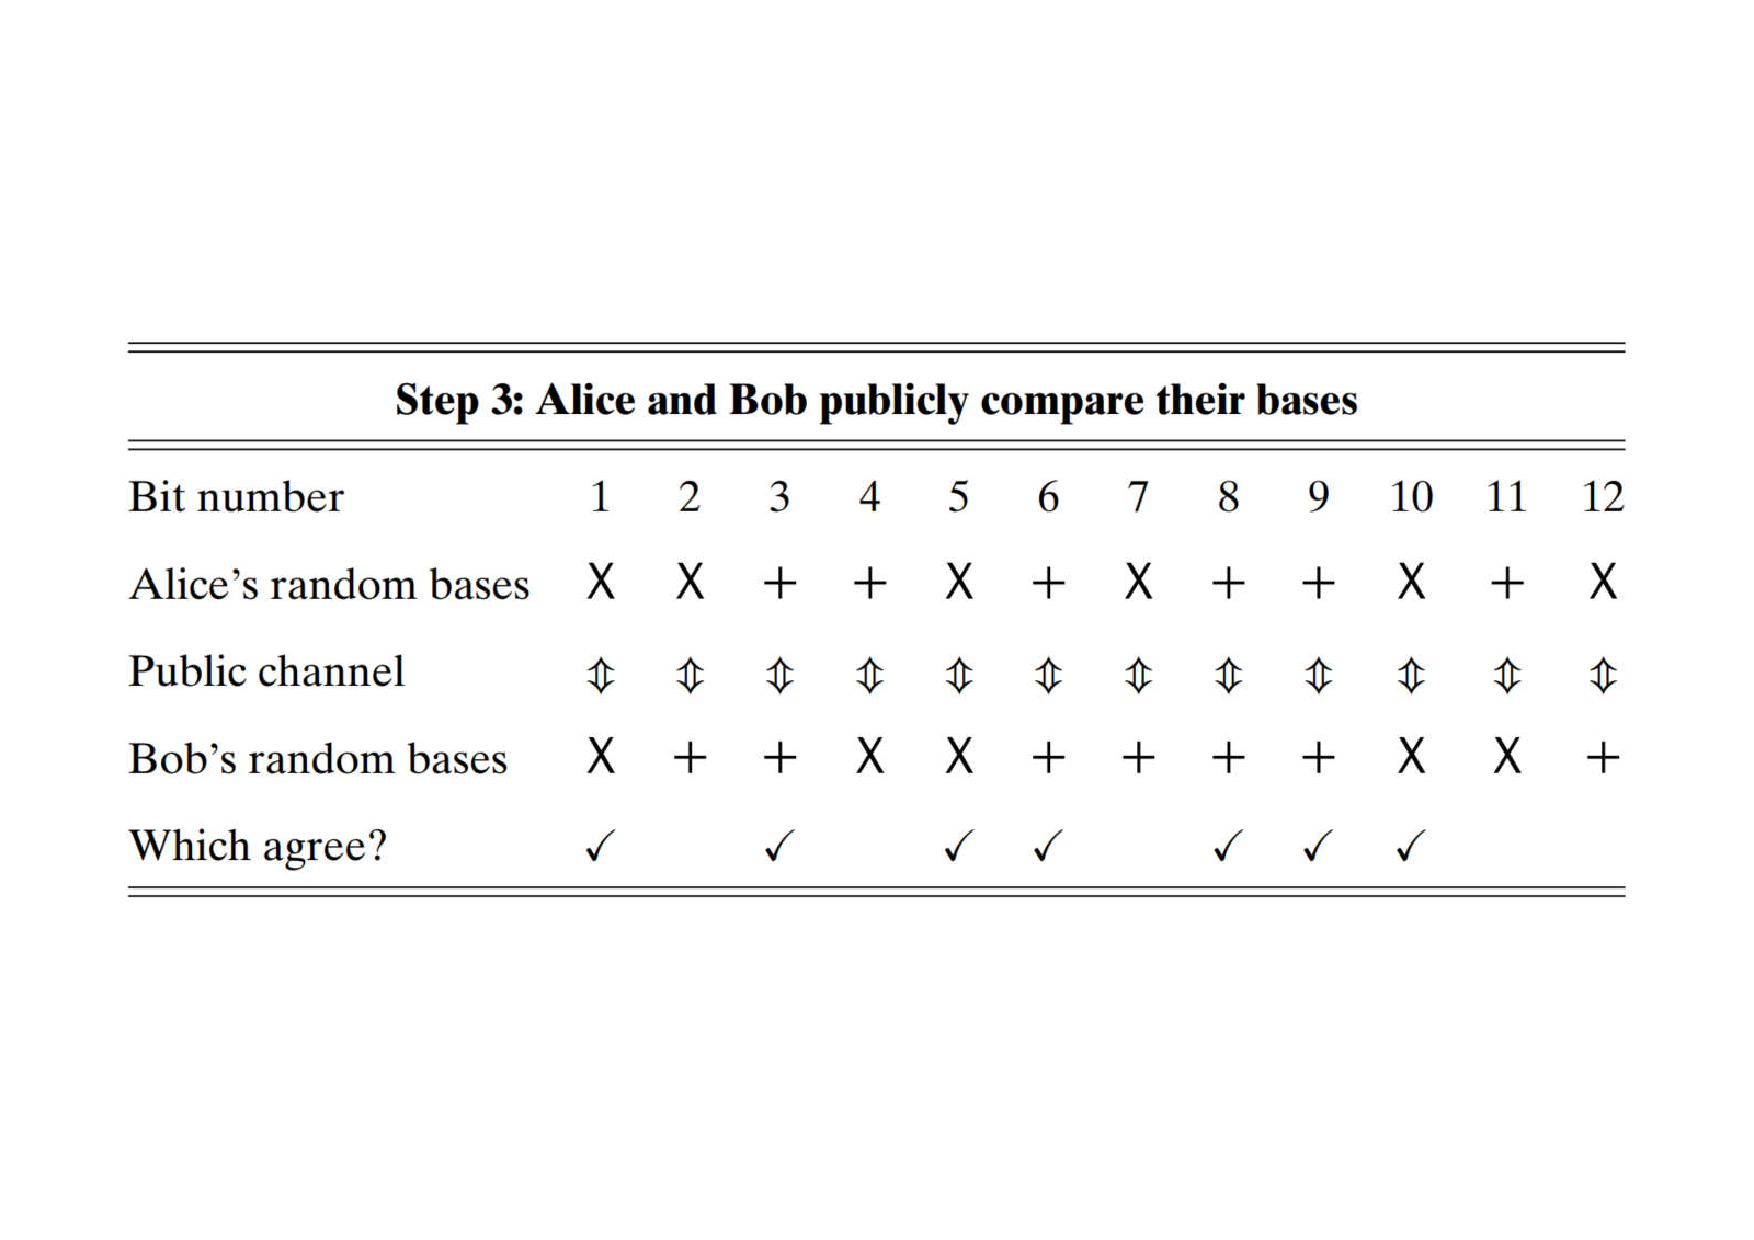
\includegraphics[width=0.75\textwidth]{BB84-step3}
				\label{fig:BB84-step3}
			\end{figure}
		\end{itemize}
	\item (Bob)
		\begin{itemize}
			\item randomly chooses half of the $n/2$ bits
			\item publicly compares them with Alice
			\begin{figure}[h]
				\centering
				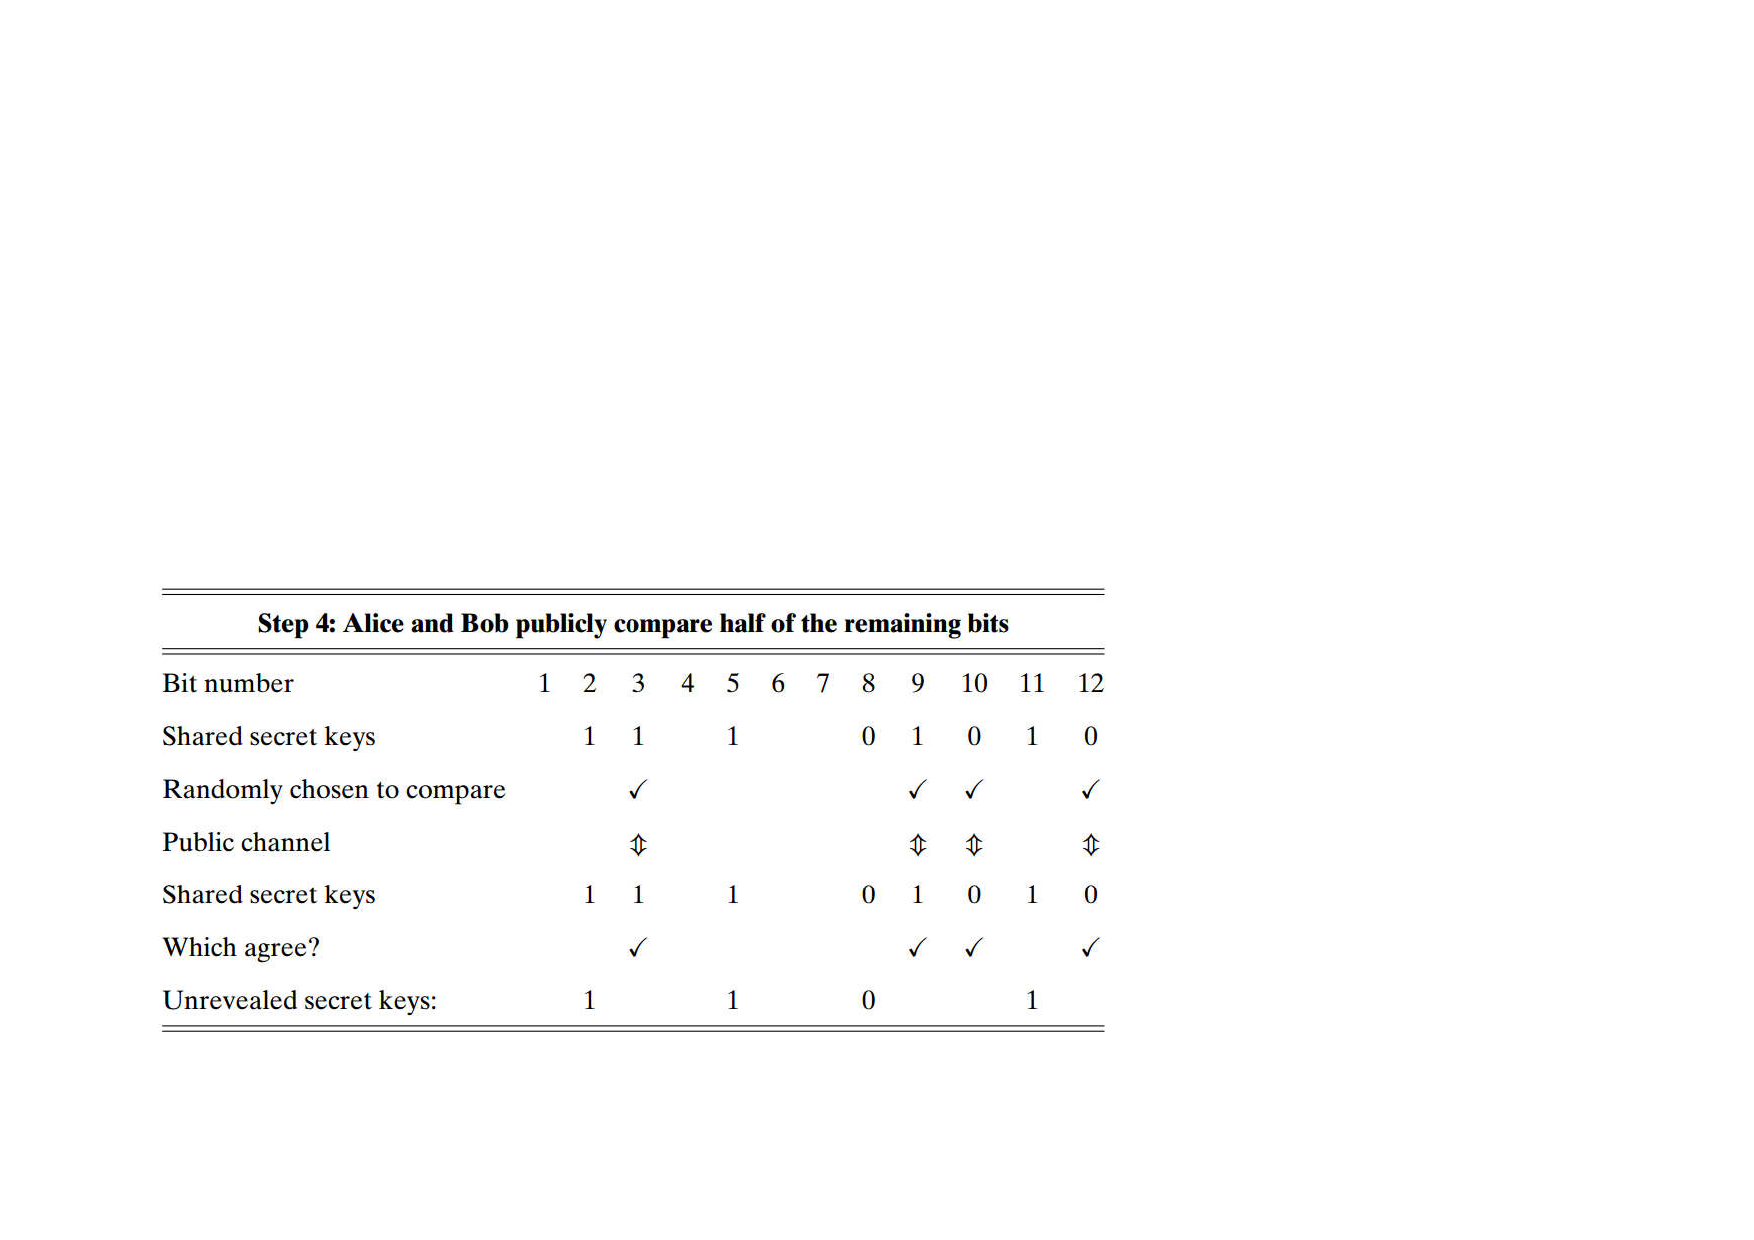
\includegraphics[width=0.75\textwidth]{BB84-step4}
				\label{fig:BB84-step4}
			\end{figure}

			If $\textrm{ECR}\leq 1-\epsilon$, Eve is listening, Alice and Bob scratch the whole sequence. Otherwise, Alice and Bob scratch out the revealed test subsequence and keep the remains as unrevealed secret private key.			
		\end{itemize}
\end{enumerate}


\subsection{The B92 protocol}
In the BB84 protocol, Alice had two distinct orthogonal bases at her disposal. It turns out that the use of two different bases is redundant, provided one employs a slightly slicker means of measuring. This simplification results in another quantum key distribution protocol, known as B92, invented by Charles Bennett in 1992.

\textbf{The non-orthogonal basis.} Alice uses only one non-orthogonal basis 
\begin{equation}
	\{\ket{\rightarrow},\ket{\nearrow}\}=\big{\{}[1,0]^{\top},\frac{1}{\sqrt{2}}[1,1]^{\top}\big{\}}
\end{equation}

\textbf{B92 protocol.} There are totally $4$ steps in the B92 protocol:
\begin{enumerate}[\textbf{step} 1]
	\item (Alice) 
		\begin{itemize}
			\item randomly determine classical bits to send
			\item send the bits in the appropriate polarization
			\begin{figure}[h]
				\centering
				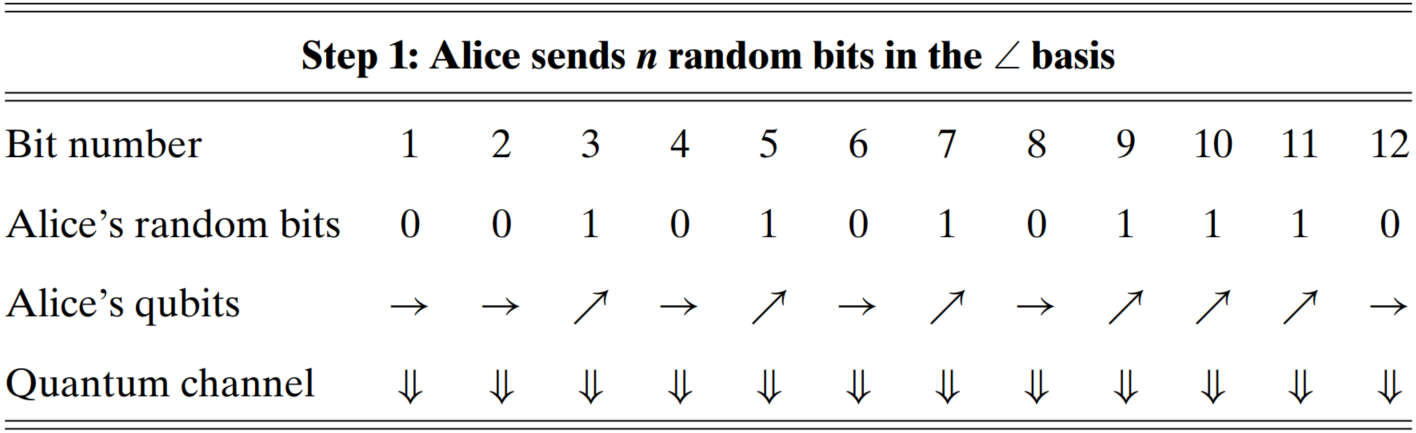
\includegraphics[width=0.75\textwidth]{B92-step1}
				\label{fig:B92-step1}
			\end{figure}
		\end{itemize}
	
	\item (Bob)
		\begin{itemize}
			\item randomly determine the bases to receive bits
			\item measure the qubit in those random bases 
			
			\begin{figure}[h]
				\centering
				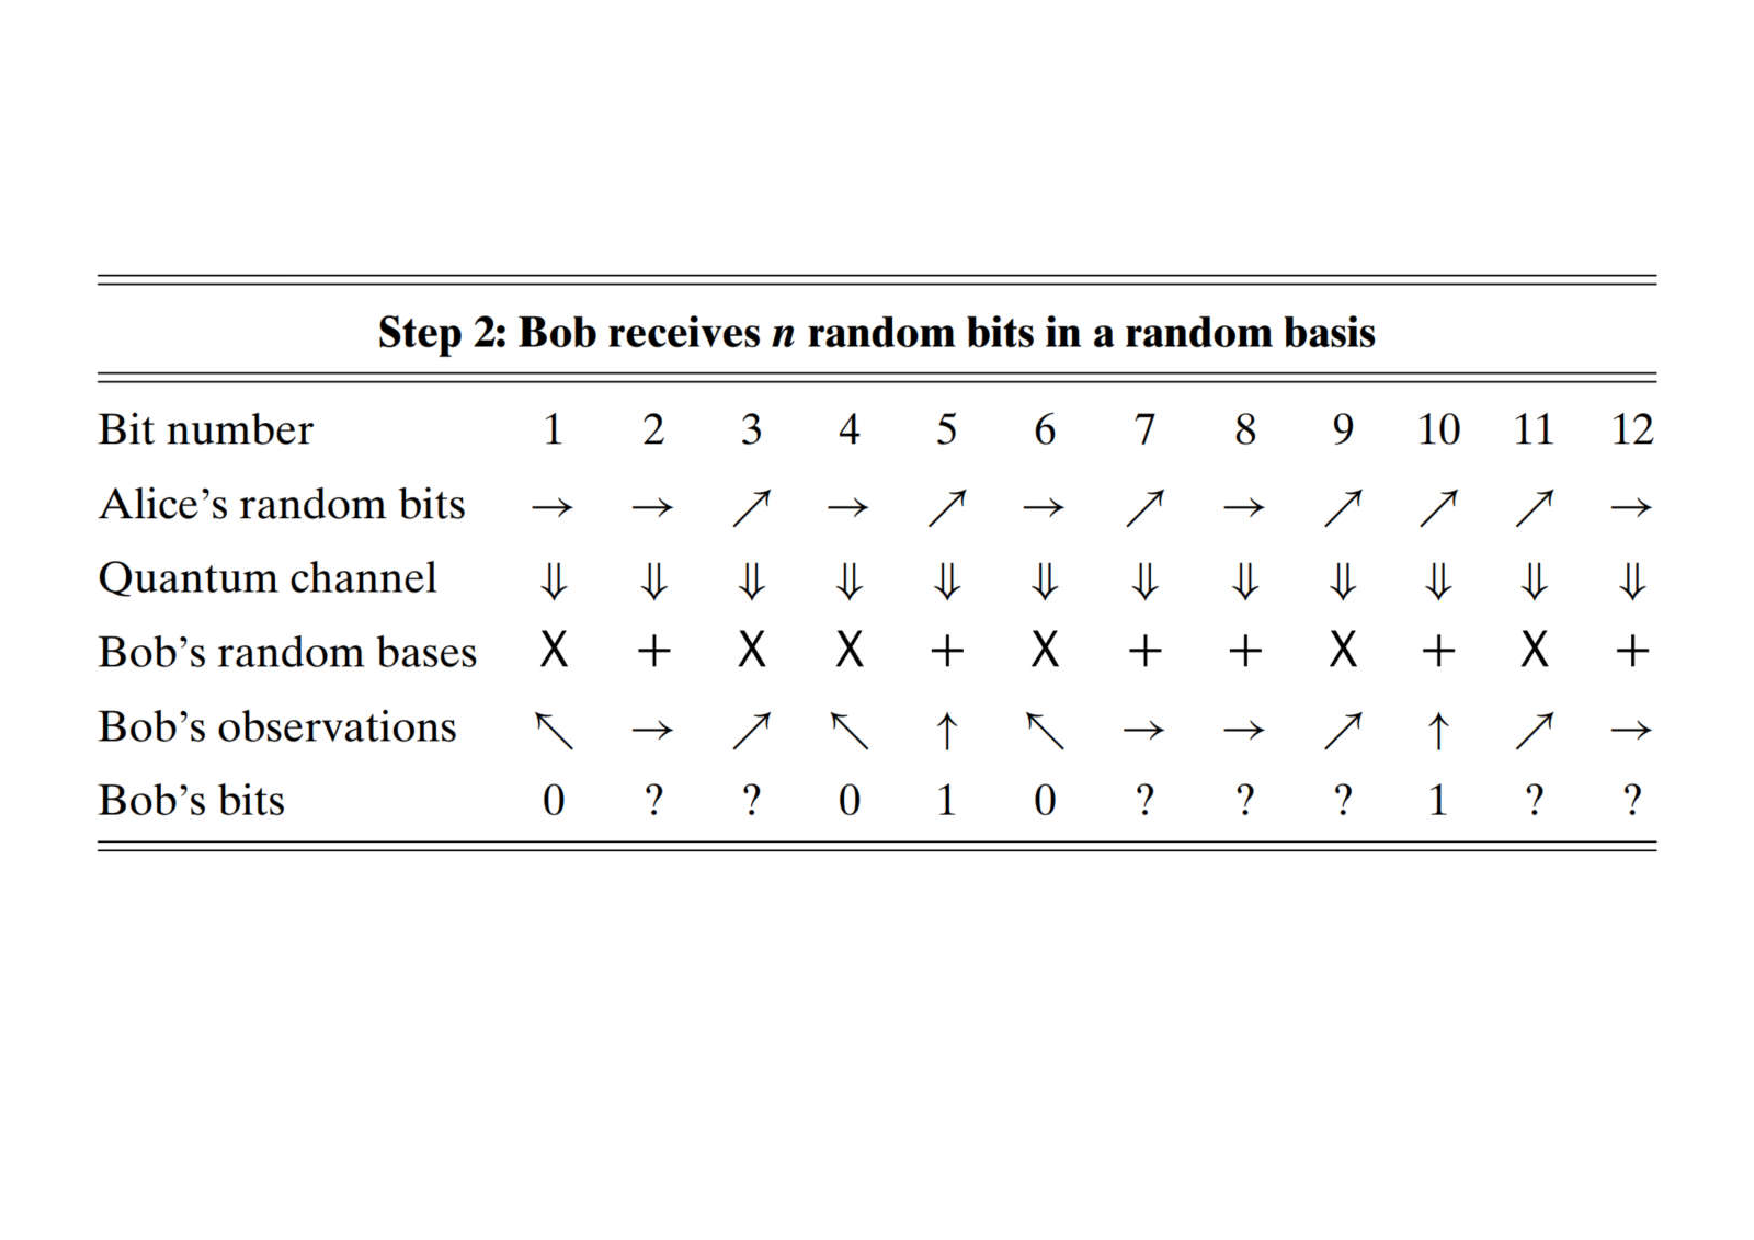
\includegraphics[width=0.75\textwidth]{B92-step2}
				\label{fig:B92-step2}
			\end{figure}
		
			\begin{itemize}
				\item If Bob uses the $+$ basis and observes a $\ket{\uparrow}$, then he knows that Alice must have sent a $\ket{\nearrow}=\ket{1}$ because if Alice had sent a $\ket{\rightarrow}$, Bob would have received a $\ket{\rightarrow}$.
				
				\item If Bob uses the $+$ basis and observes a $\ket{\rightarrow}$, then it is not clear to him which qubit Alice sent. She could have sent a $\ket{\rightarrow}$ but she could also have sent a $\ket{\nearrow}$
				that collapsed to a $\ket{\rightarrow}$. Because Bob is in doubt, he will omit this bit.
				
				\item If Bob uses the $\times$ basis and observes a $\ket{\nwarrow}$, then he knows that Alice must have sent a $\ket{\rightarrow}=\ket{0}$ because if Alice had sent a $\ket{\nearrow}$, Bob would have received a $\ket{\nearrow}$.
				
				\item If Bob uses the $\times$ basis and observes a $\ket{\nearrow}$, then it is not clear to him which qubit Alice sent. She could have sent a $\ket{\nearrow}$ but she could also have sent a $\ket{\rightarrow}$ that collapsed to a $\ket{\nearrow}$. Because Bob is in doubt, he will omit this bit.
			\end{itemize}
		\end{itemize}
	
	\item (Alice and Bob)
		\begin{itemize}
			\item Bob publicly tells Alice which bits were uncertain 
			\item they both omit uncertain bits
		\end{itemize}
	
	\item (optional for intrusion detection)	
		\begin{itemize}
			\item Bob randomly chooses half of the $n/2$ bits
			\item Bob publicly compares them with Alice
		\end{itemize}
\end{enumerate}


\subsection{The EPR protocol}
In 1991, Artur K. Ekert proposed a completely different type of quantum key distribution protocol based on entanglement. In the chapter of composite system, we learned that we can prepare a sequence of entangled pairs of qubits like $\frac{\ket{00}+\ket{11}}{\sqrt{2}}$ or $\frac{\ket{01}+\ket{10}}{\sqrt{2}}$. For the discussion convenience, we assume the pair of entangled qubits in the state of $\frac{\ket{00}+\ket{11}}{\sqrt{2}}$.

\begin{enumerate}[\textbf{step} 1]
	\item (Alice and Bob) 
		\begin{itemize}
			\item Both sides are each assigned one of each of the pairs of entangled qubits 
		\end{itemize}
	
	\item (Alice and Bob)
		\begin{itemize}
			\item separately choose a random sequence of bases 
			\item measure their qubits in their chosen basis 
			\begin{figure}[h]
				\centering
				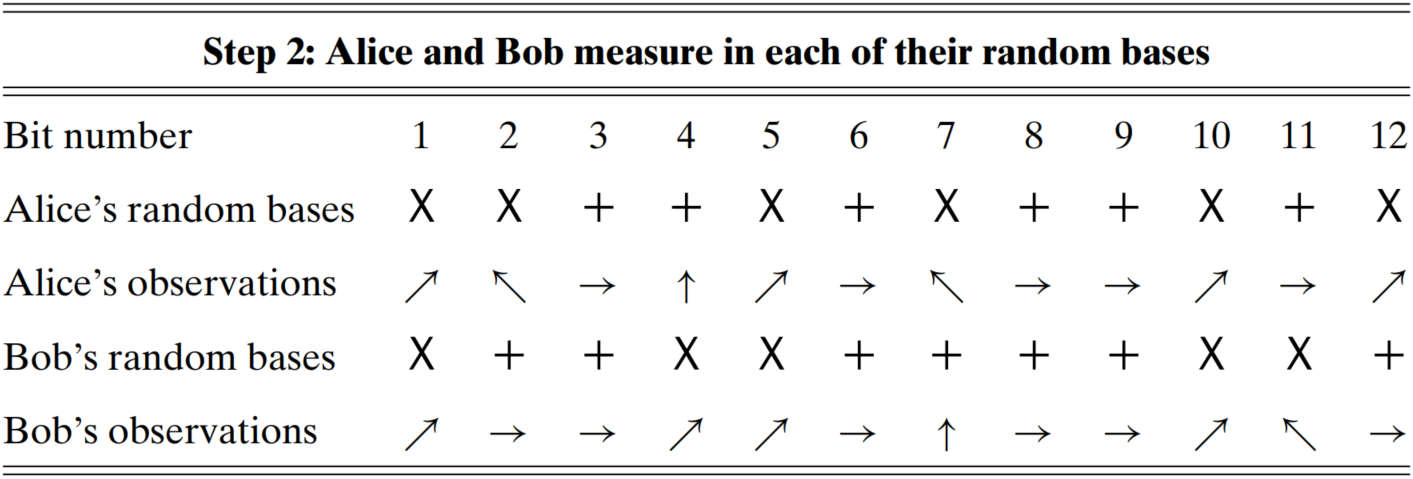
\includegraphics[width=0.75\textwidth]{EPR-step2}
				\label{fig:EPR-step2}
			\end{figure}
		\end{itemize}
	
	\item (Alice and Bob)
		\begin{itemize}
			\item publicly compare what bases were used  
			\item keep only those bits measured in the same basis
			\begin{figure}[h]
				\centering
				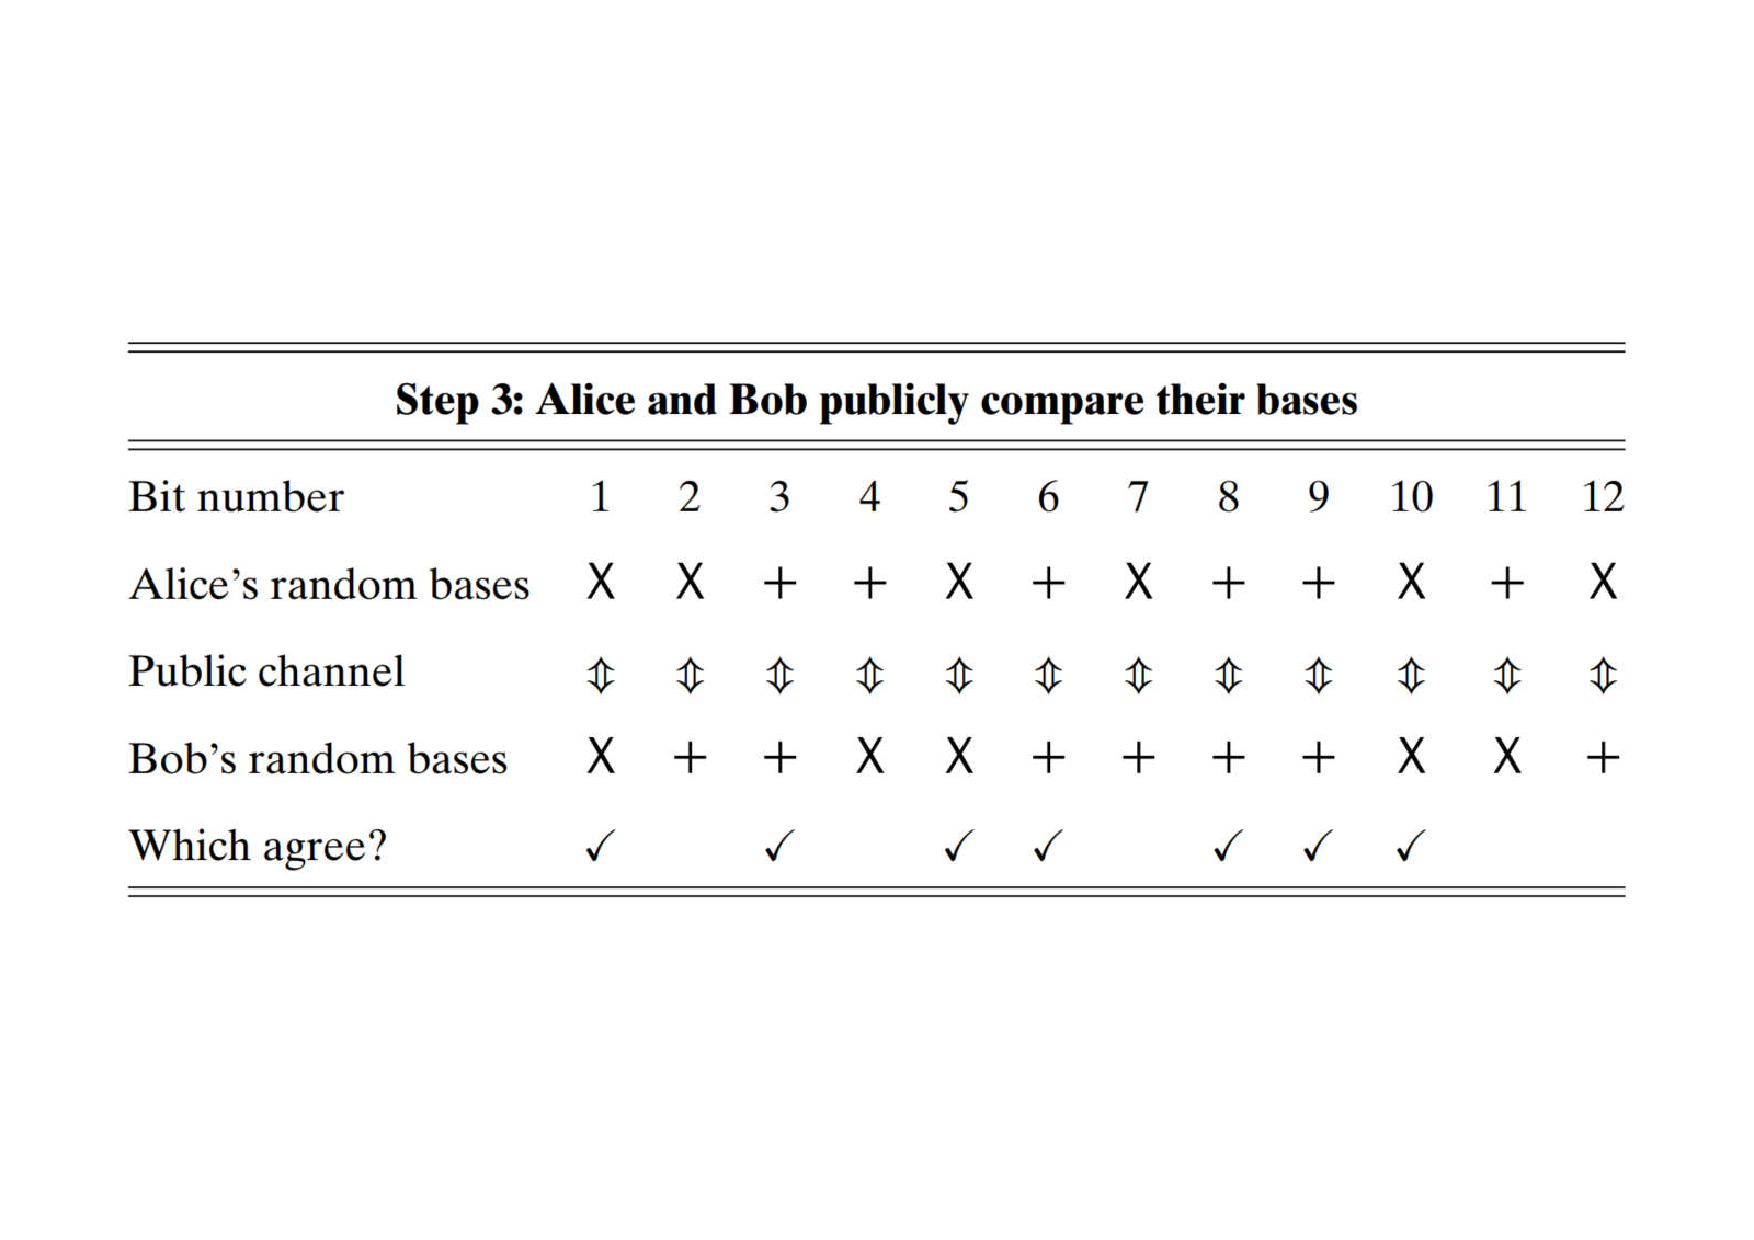
\includegraphics[width=0.75\textwidth]{EPR-step3}
				\label{fig:EPR-step3}
			\end{figure}
		\end{itemize}	
	
	\item (optional for intrusion or disentangled detection)
		\begin{itemize}
			\item Bob randomly chooses half of the n/2 bits  
			\item Bob publicly compares them with Alice
		\end{itemize}
	
\end{enumerate}


\section{Quantum Teleportation}
\textbf{Quantum teleportation} is the process by which the state of an arbitrary qubit is transferred from one location to another.

\textbf{Canonical and non-canonical bases for a single qubit.} When working with a single qubit, we worked with the canonical basis, $\{\ket{0},\ket{1}\}$, and non-canonical basis, $\{\frac{\ket{0}+\ket{1}}{\sqrt{2}}, \frac{\ket{0}-\ket{1}}{\sqrt{2}}\}$, as shown in Figure \ref{fig:canonical-non-canonical-bases}. 

\begin{figure}[h]
	\centering
	\subfloat[The canonical base]
	{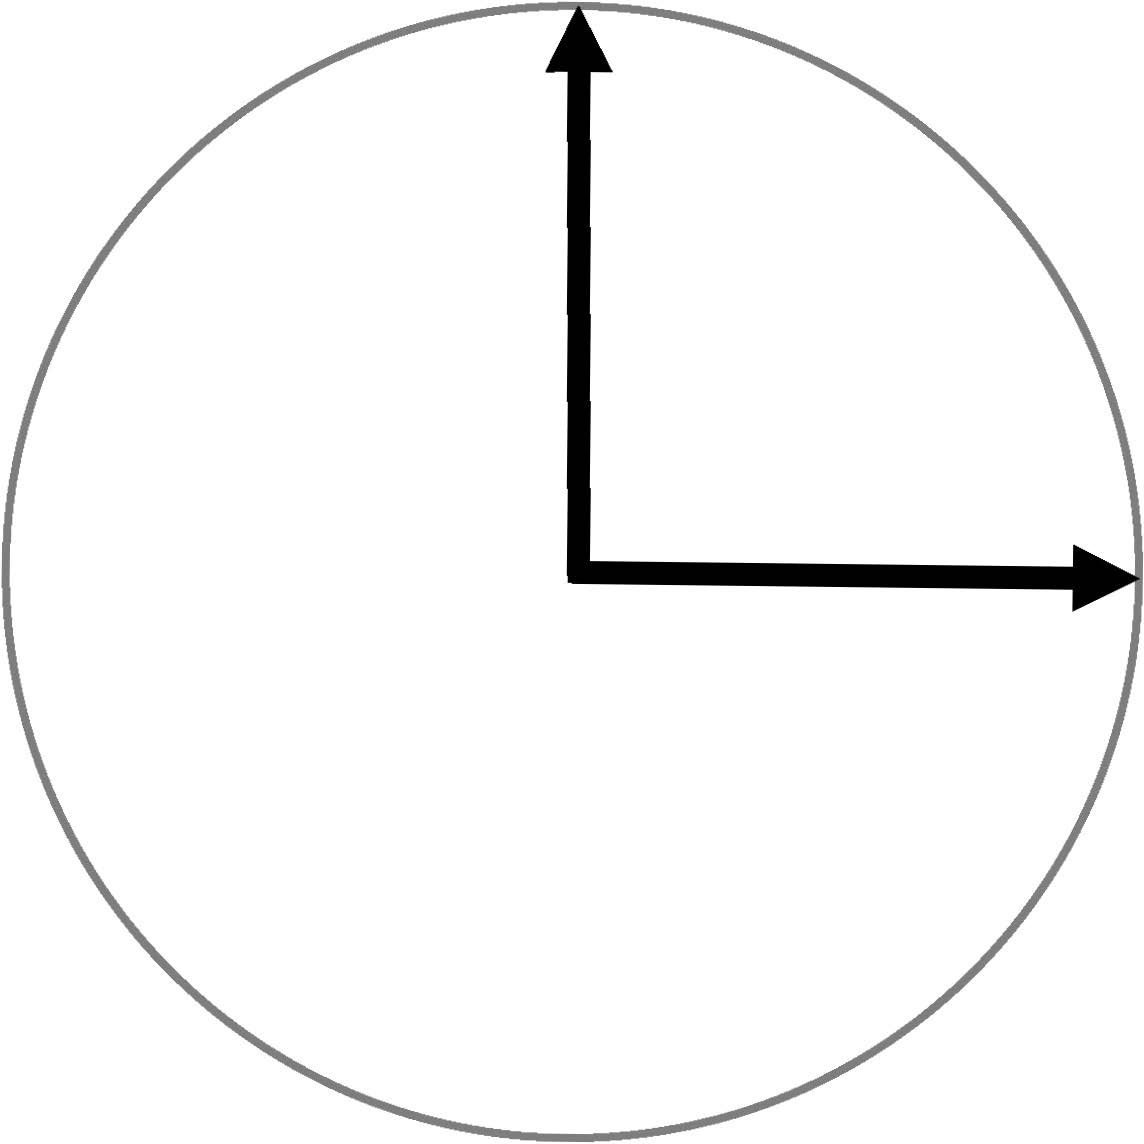
\includegraphics[width=0.3\textwidth]{canonical-basis}
		\label{subfig:canonical-basis}}
	\hspace{0.2\textwidth}
	\subfloat[The non-canonical base]
	{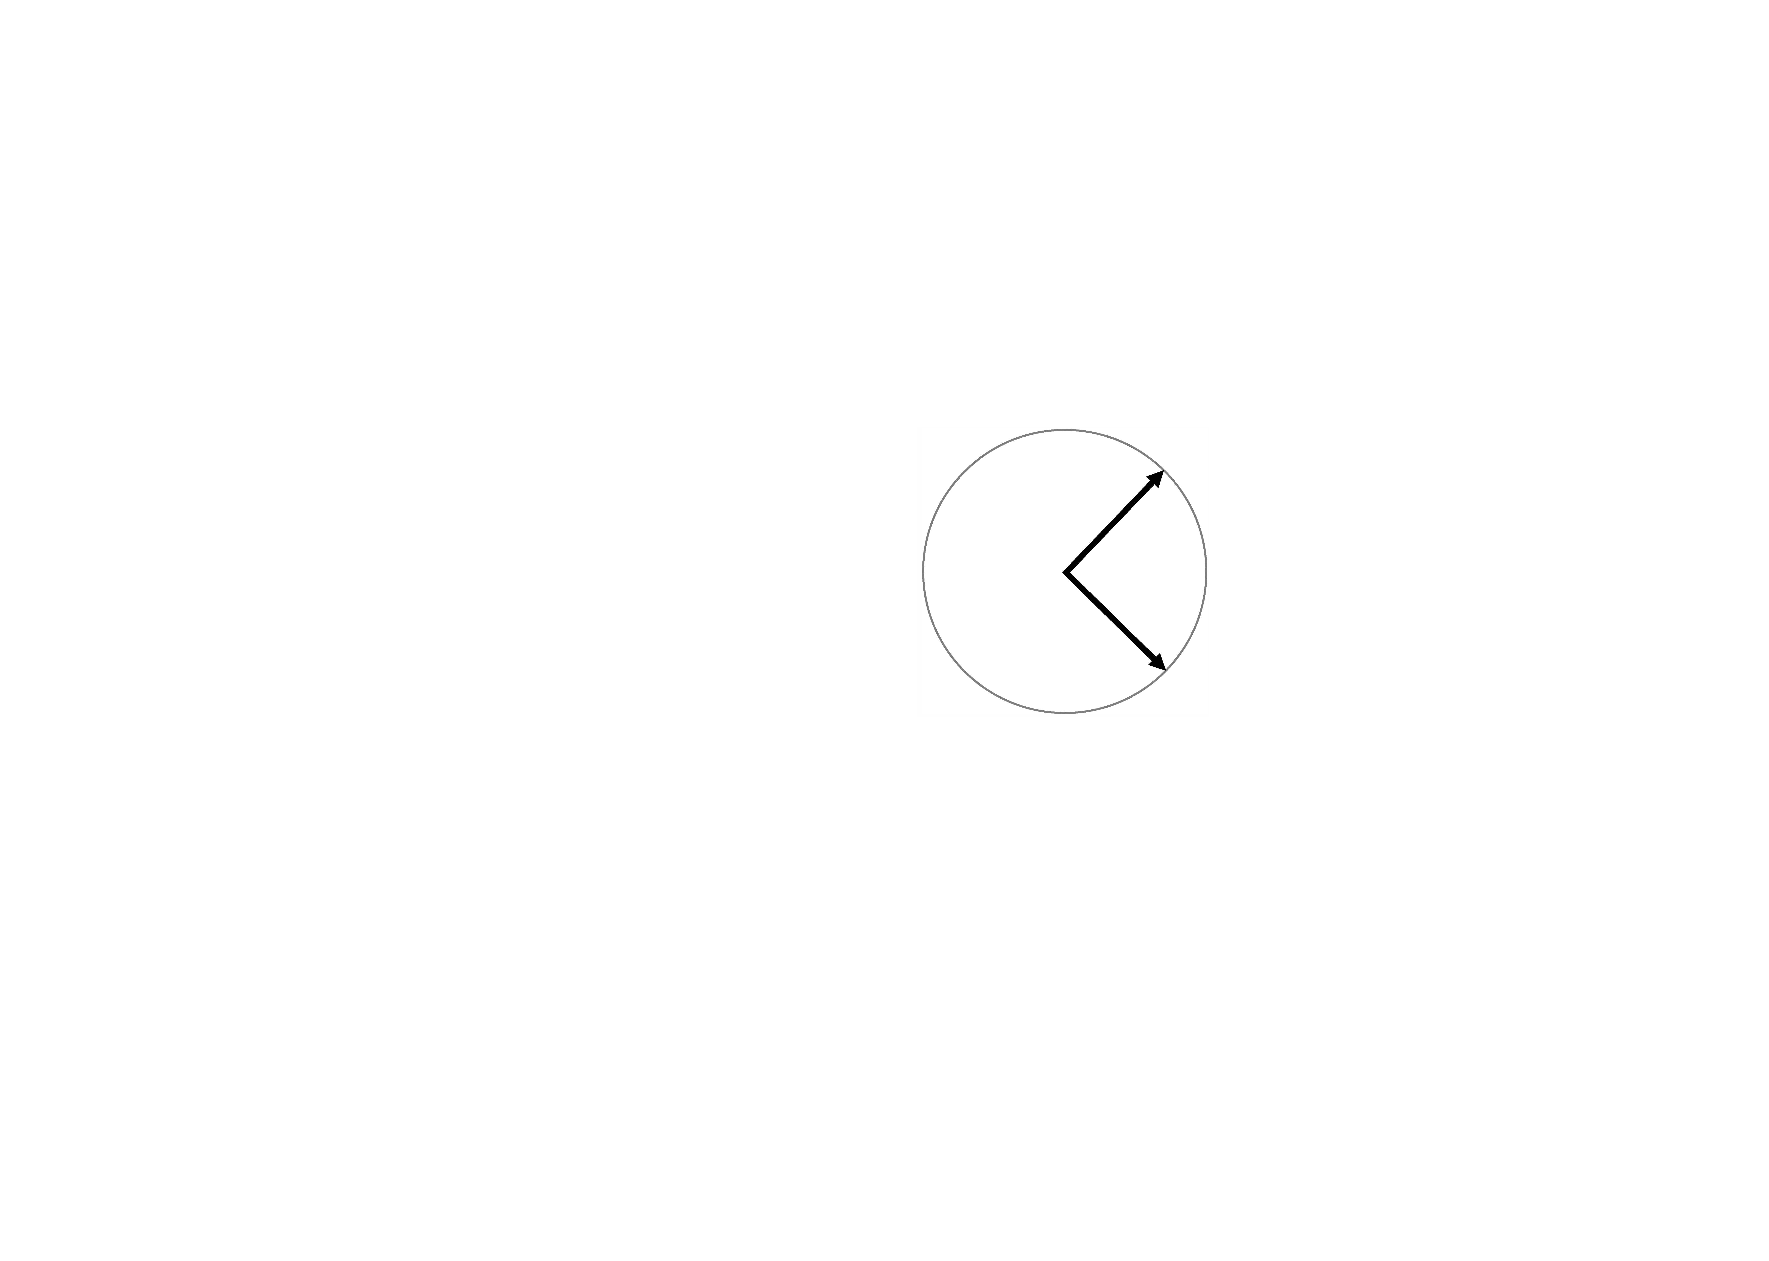
\includegraphics[width=0.3\textwidth]{non-canonical-basis}
		\label{subfig:non-canonical-basis}}
	\caption{Canonical and non-canonical basis used in the quantum teleportation.}
	\label{fig:canonical-non-canonical-bases}
\end{figure}

\textbf{Canonical and non-canonical bases for two qubits.} The teleportation algorithm will work with two entangled qubits, one held by Alice and one held by Bob. The obvious canonical basis for this four-dimensional space is:
\begin{equation}
	\{\ket{0_A 0_B}, \ket{0_A 1_B}, \ket{1_A 0_B}, \ket{1_A 1_b}\}
\end{equation}
A non-canonical basis, called the Bell basis in honor of John Bell, consists of the
following four vectors:
\begin{equation}
	\begin{aligned}
		\ket{\Psi^+}&=\frac{\ket{0_A 1_B}+\ket{1_A 0_B}}{\sqrt(2)},\quad
		\ket{\Psi^-}=\frac{\ket{0_A 1_B}-\ket{1_A 0_B}}{\sqrt(2)},\\
		\ket{\Phi^+}&=\frac{\ket{0_A 0_B}+\ket{1_A 1_B}}{\sqrt(2)},\quad
		\ket{\Phi^-}=\frac{\ket{0_A 0_B}-\ket{1_A 1_B}}{\sqrt(2)}
	\end{aligned}
\end{equation}
Every vector in this basis is entangled.

\textbf{Bell circuit.} How to derive the Bell basis? In the single qubit (two-dimensional) case, the elements of the noncanonical basis can be formed using the Hadamard matrix:
\begin{equation}
	\mathbf{H}\ket{0} = \frac{\ket{0}+\ket{1}}{\sqrt{2}}\quad \textrm{and}\quad \mathbf{H}\ket{1} = \frac{\ket{0}-\ket{1}}{\sqrt{2}}
\end{equation}

In the two qubits (four-dimensional) case, the elements of the non-canonical basis are derived from Bell circuit:
\begin{figure}[h]
	\centering
	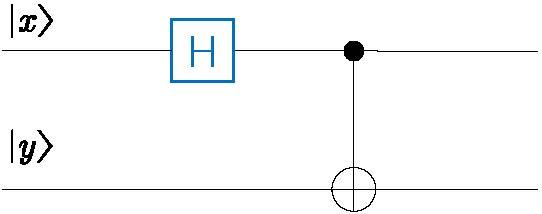
\includegraphics[width=0.5\textwidth]{Bell-circuit}
	\label{fig:Bell-circuit}
\end{figure}

From which, we have $\ket{00}\mapsto\ket{\Phi^+}$, $\ket{10}\mapsto\ket{\Phi^-}$, $\ket{01}\mapsto\ket{\Psi^+}$, $\ket{11}\mapsto\ket{\Psi^-}$.

\begin{example}[$\ket{00}\mapsto\ket{\Phi^+}$]{ex:Bell-circuit}
	\begin{equation}
		\begin{aligned}
			\textrm{CNOT}\cdot(\mathbf{H}\ket{0}\otimes \ket{0})&=\textrm{CNOT}\cdot(\frac{\ket{0}+\ket{1}}{\sqrt{2}}\otimes \ket{0})\\&=
			\begin{bmatrix}
				1 & 0 & 0 & 0\\
				0 & 1 & 0 & 0\\
				0 & 0 & 1 & 0\\
				0 & 0 & 0 & 1
			\end{bmatrix}\cdot\frac{1}{\sqrt{2}}
			\begin{bmatrix}
				1\\0\\1\\0
			\end{bmatrix}=\frac{1}{\sqrt{2}}
			\begin{bmatrix}
				1\\0\\0\\1
			\end{bmatrix}=\frac{\ket{00}+\ket{11}}{\sqrt{2}}=\ket{\Phi^+}
		\end{aligned}
	\end{equation} 
\end{example}

\textbf{Quantum teleportation protocol.} The whole protocol contains $5$ steps:

\begin{enumerate}[\textbf{step} 1]
	\item : Alice has a qubit $\ket{\psi}=\alpha\ket{0}+\beta\ket{1}$.
	
	\item : prepare two entangled quibit A and B
		\begin{itemize}
			\item two entangled quibits are formed as $\ket{\Phi^+}$
			\item one is given to Alice and one is given to Bob
		\end{itemize}
		\begin{figure}[h]
			\centering
			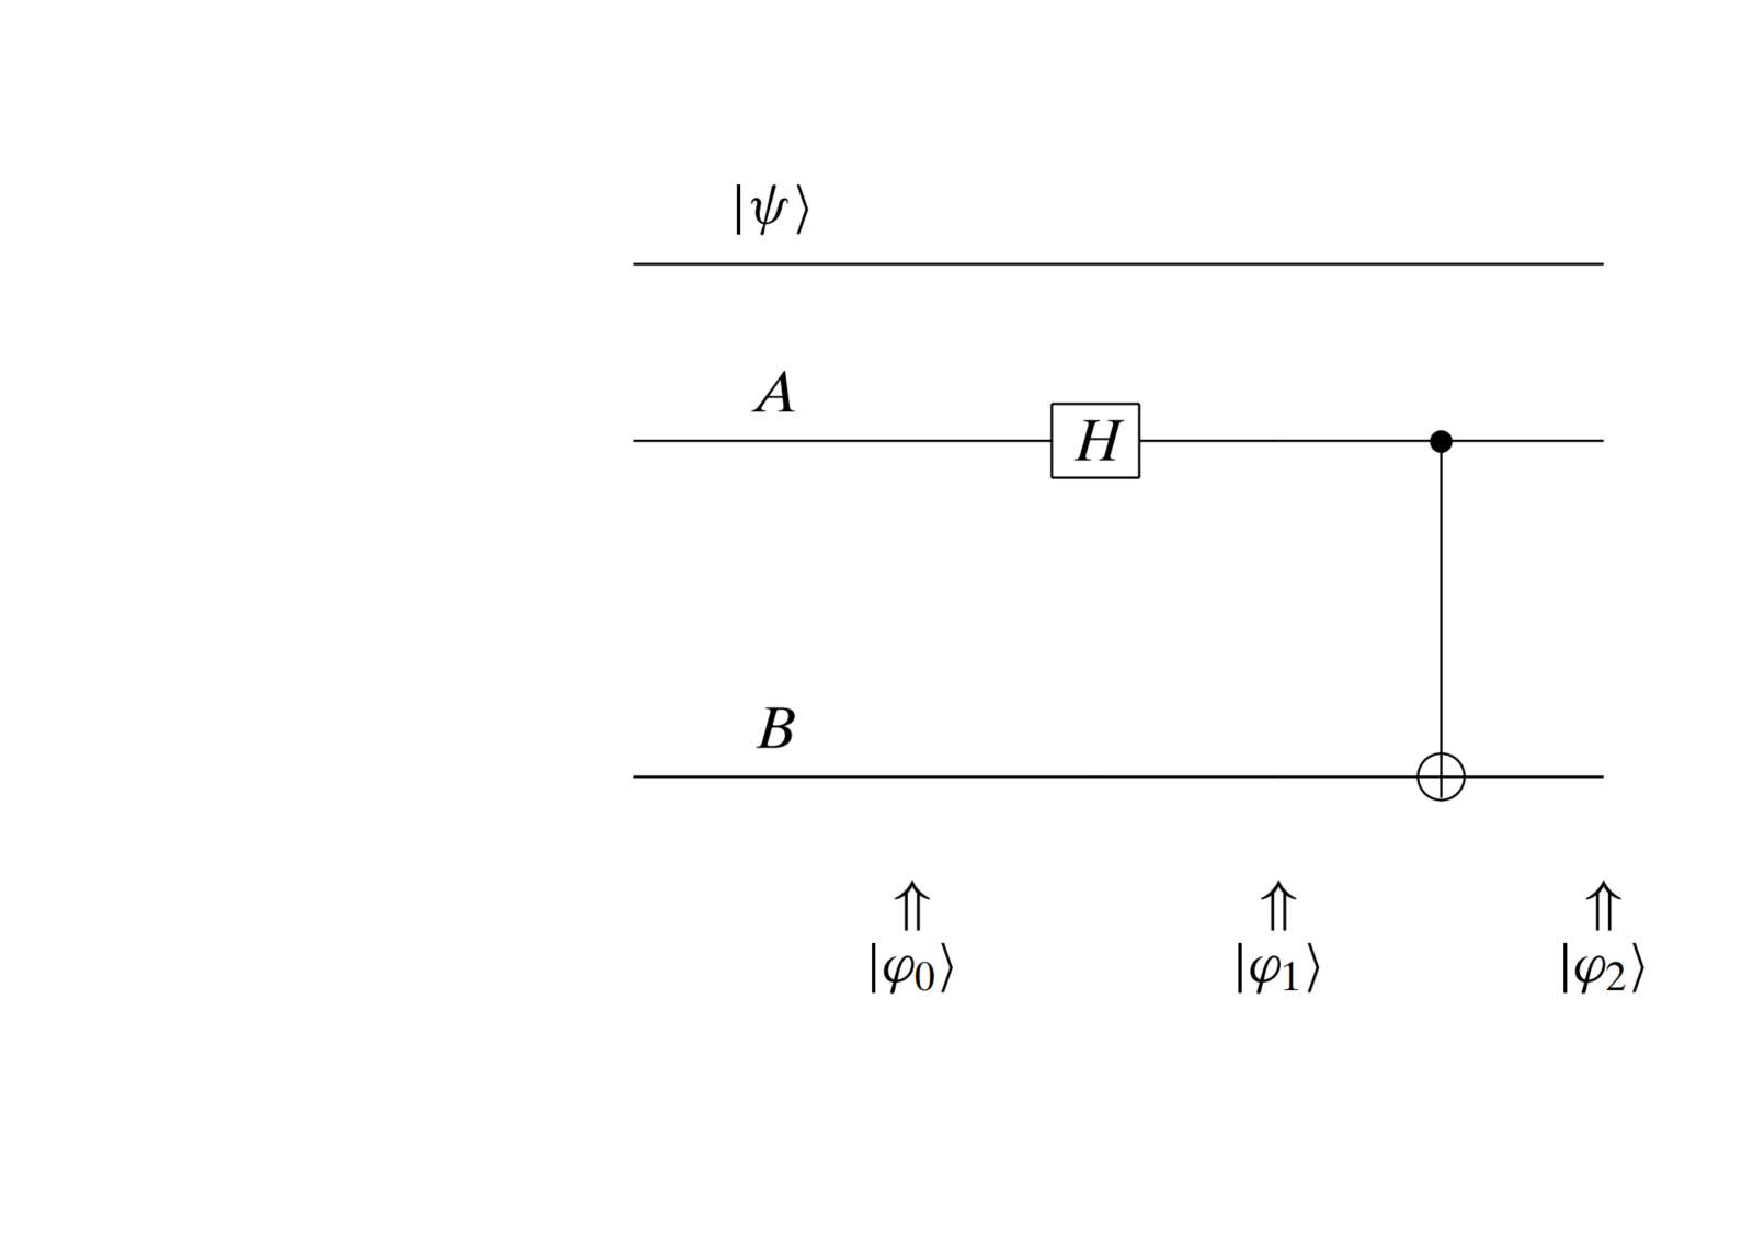
\includegraphics[width=0.45\textwidth]{qt-step2}
			\label{fig:qt-step2}
		\end{figure}
	
		\begin{equation}
			\begin{aligned}
				\ket{\varphi_0}&=\ket{\psi}\otimes\ket{0_A}\otimes\ket{0_B}=\ket{\psi}\ket{0_A 0_B}\\
				\ket{\varphi_1}&=\ket{\psi}\otimes\frac{\ket{0_A}+\ket{1_A}}{\sqrt{2}}\otimes\ket{0_B}\\
				\ket{\varphi_2}&=\ket{\psi}\otimes\ket{\Phi^+}=\ket{\psi}\otimes\frac{\ket{0_A 0_B}+\ket{1_A 1_B}}{\sqrt{2}}\\
				&=(\alpha\ket{0}+\beta\ket{1})\otimes\frac{\ket{0_A 0_B}+\ket{1_A 1_B}}{\sqrt{2}}\\
				&=\frac{\alpha\ket{}(\ket{0_A 0_B}+\ket{1_A 1_B})+\beta\ket{1}(\ket{0_A 0_B}+\ket{1_A 1_B})}{\sqrt{2}}
			\end{aligned}
		\end{equation}
		
	
	\item : Alice lets her $\ket{\psi}$ interact with her entangled qubit
	\begin{figure}[h]
		\centering
		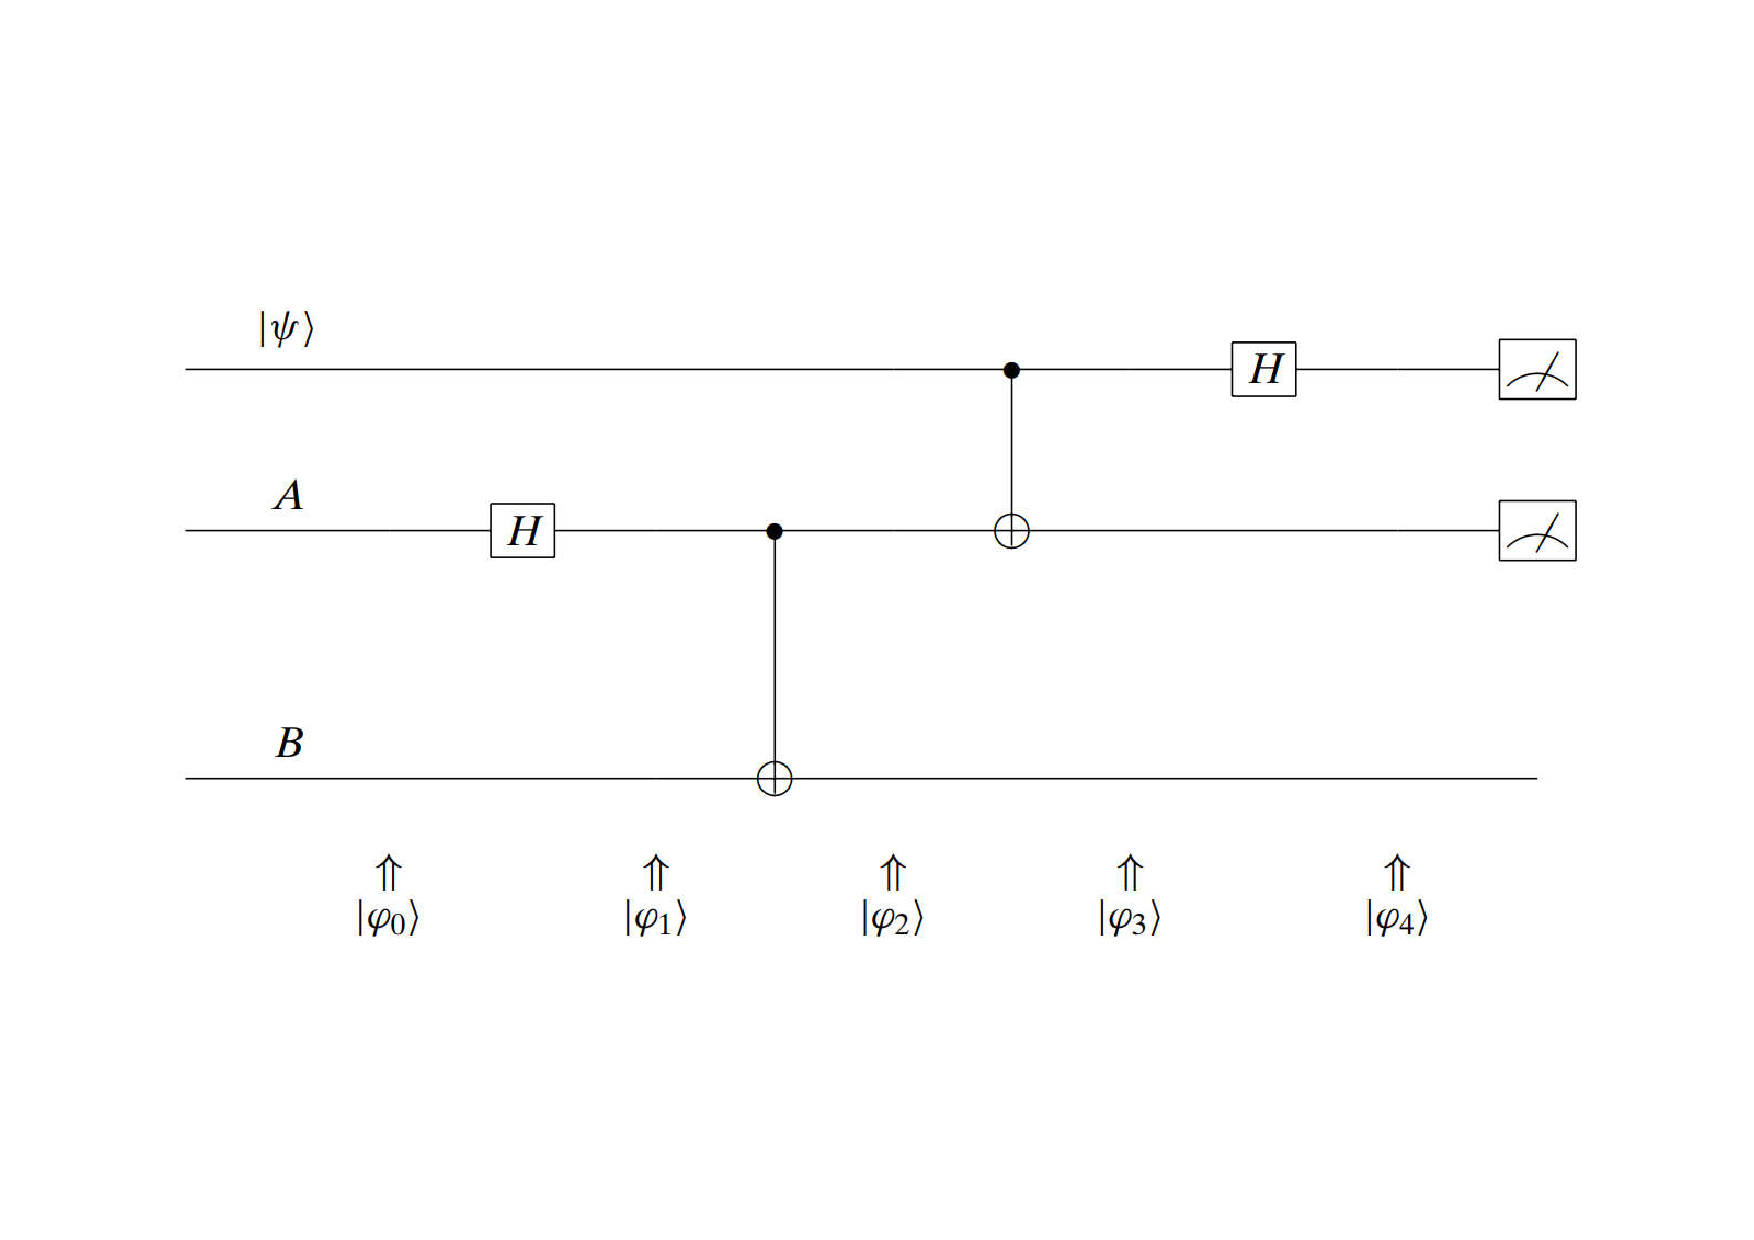
\includegraphics[width=0.8\textwidth]{qt-step3}
		\label{fig:qt-step3}
	\end{figure}
	
	\begin{equation}
		\begin{aligned}
			\ket{\varphi_2}&=\frac{\alpha\ket{0}(\ket{0_A 0_B}+\ket{1_A 1_B})+\beta\ket{1}(\ket{0_A 0_B}+\ket{1_A 1_B})}{\sqrt{2}}\\
			\ket{\varphi_3}&=\frac{\alpha\ket{0}(\ket{0_A 0_B}+\ket{1_A 1_B})+\beta\ket{1}(\ket{1_A 0_B}+\ket{0_A 1_B})}{\sqrt{2}}\\
			\ket{\varphi_4}&=\frac{1}{2}(\alpha(\ket{0}+\ket{1})(\ket{0_A 0_B}+\ket{1_A 1_B})+\beta(\ket{0}-\ket{1})(\ket{1_A 0_B}+\ket{0_A 1_B}))\\
			&=\frac{1}{2}(\alpha(\ket{000}+\ket{011}+\ket{100}+\ket{111})+\beta(\ket{010}+\ket{001}-\ket{110}-\ket{101}))\\
			&=\frac{1}{2}[\ket{00}(\alpha\ket{0}+\beta\ket{1})+\ket{01}(\beta\ket{0}+\alpha\ket{1})\\
			&\quad+\ket{10}(\alpha\ket{0}-\beta\ket{1})+\ket{11}(-\beta\ket{0}+\alpha\ket{1})]
		\end{aligned}
	\end{equation}
	
	\item : Alice makes a measurement
	\begin{itemize}
		\item Alice measures her two qubits
		\item Alice determines to which of the four possible states the system collapses
	\end{itemize}

	\item : Bob performs the corresponding transformation based on Alice's observations
	\begin{itemize}
		\item Alice sends copies of her two bits (not qubits) to Bob 
		\item Bob uses that information to achieve the desired state 
		\begin{figure}[h]
			\centering
			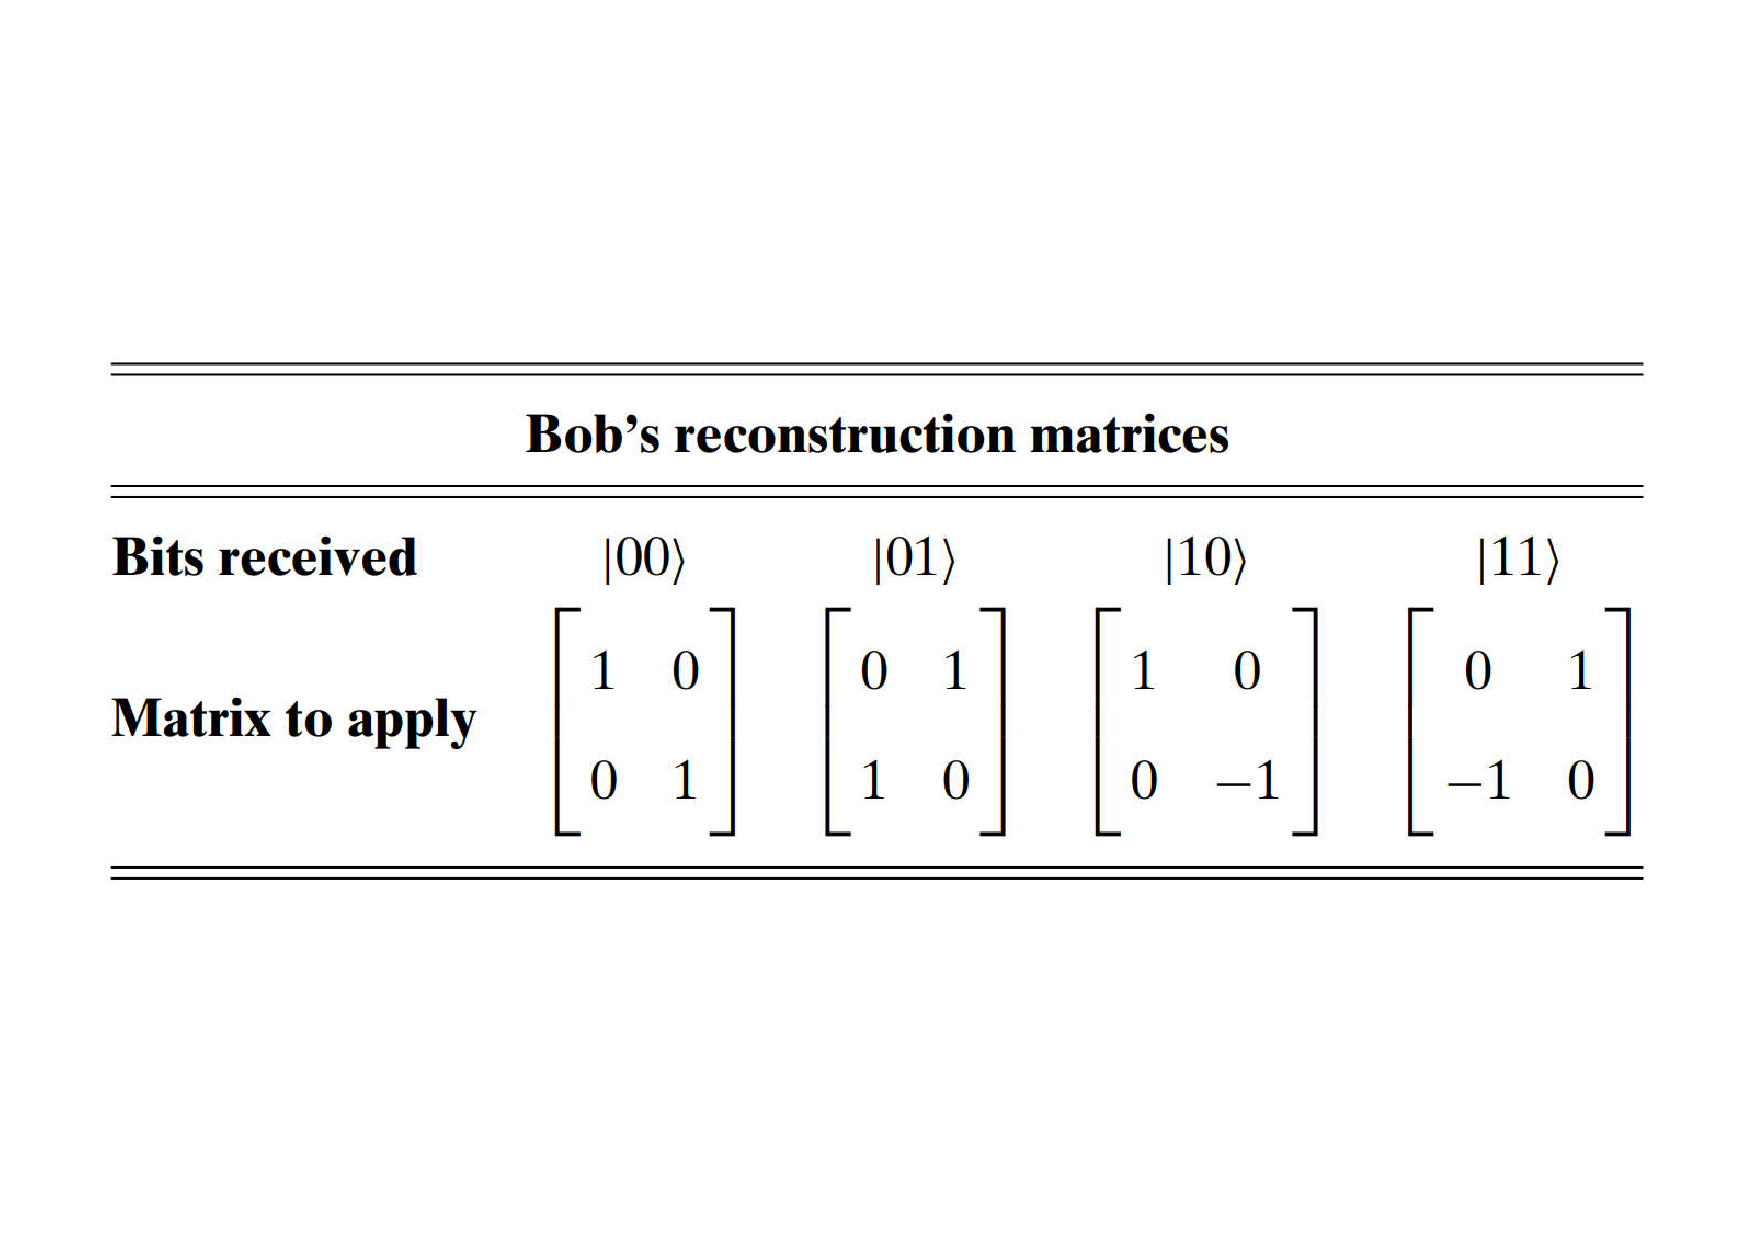
\includegraphics[width=0.6\textwidth]{qt-step5}
			\label{fig:qt-step5}
		\end{figure}
		
		\begin{example}[Bob's transformation when Alice observes $\ket{10}$]{ex:transformation}
			\begin{equation}
				\begin{bmatrix}
					1 & 0 \\
					0 & -1
				\end{bmatrix}
				\begin{bmatrix}
					\alpha\\-\beta
				\end{bmatrix}=
				\begin{bmatrix}
					\alpha\\\beta
				\end{bmatrix}=\alpha\ket{0}+\beta\ket{1}=\ket{\psi}
			\end{equation} 
		\end{example}
	\end{itemize}
\end{enumerate}

The whole framework of the quantum teleportation protocol is shown in Figure \ref{fig:qt-framework}. Several points should be made about this protocol:
\begin{itemize}
	\item Alice is no longer in possession of $\ket{\psi}$. She has only two classical bits.
	\item As we have seen, to “teleport” a single quantum particle, Alice has to send two classical bits. Without receiving them, there is no way that Bob can know what he has. These classical bits travel along a classical channel and thus they propagate at finite speed (less than the speed of light). Entanglement, in spite of its undisputable magic, does not allow you to communicate faster than the speed of light. 
	\item Information teleported from Alice to Bob via qubit is infinite, but it is useless to Bob once he make the measurement (qubit will collapse to a classic bit).
	\item no particle has been moved at all, only the state.	
\end{itemize}

\begin{figure}[h]
	\centering
	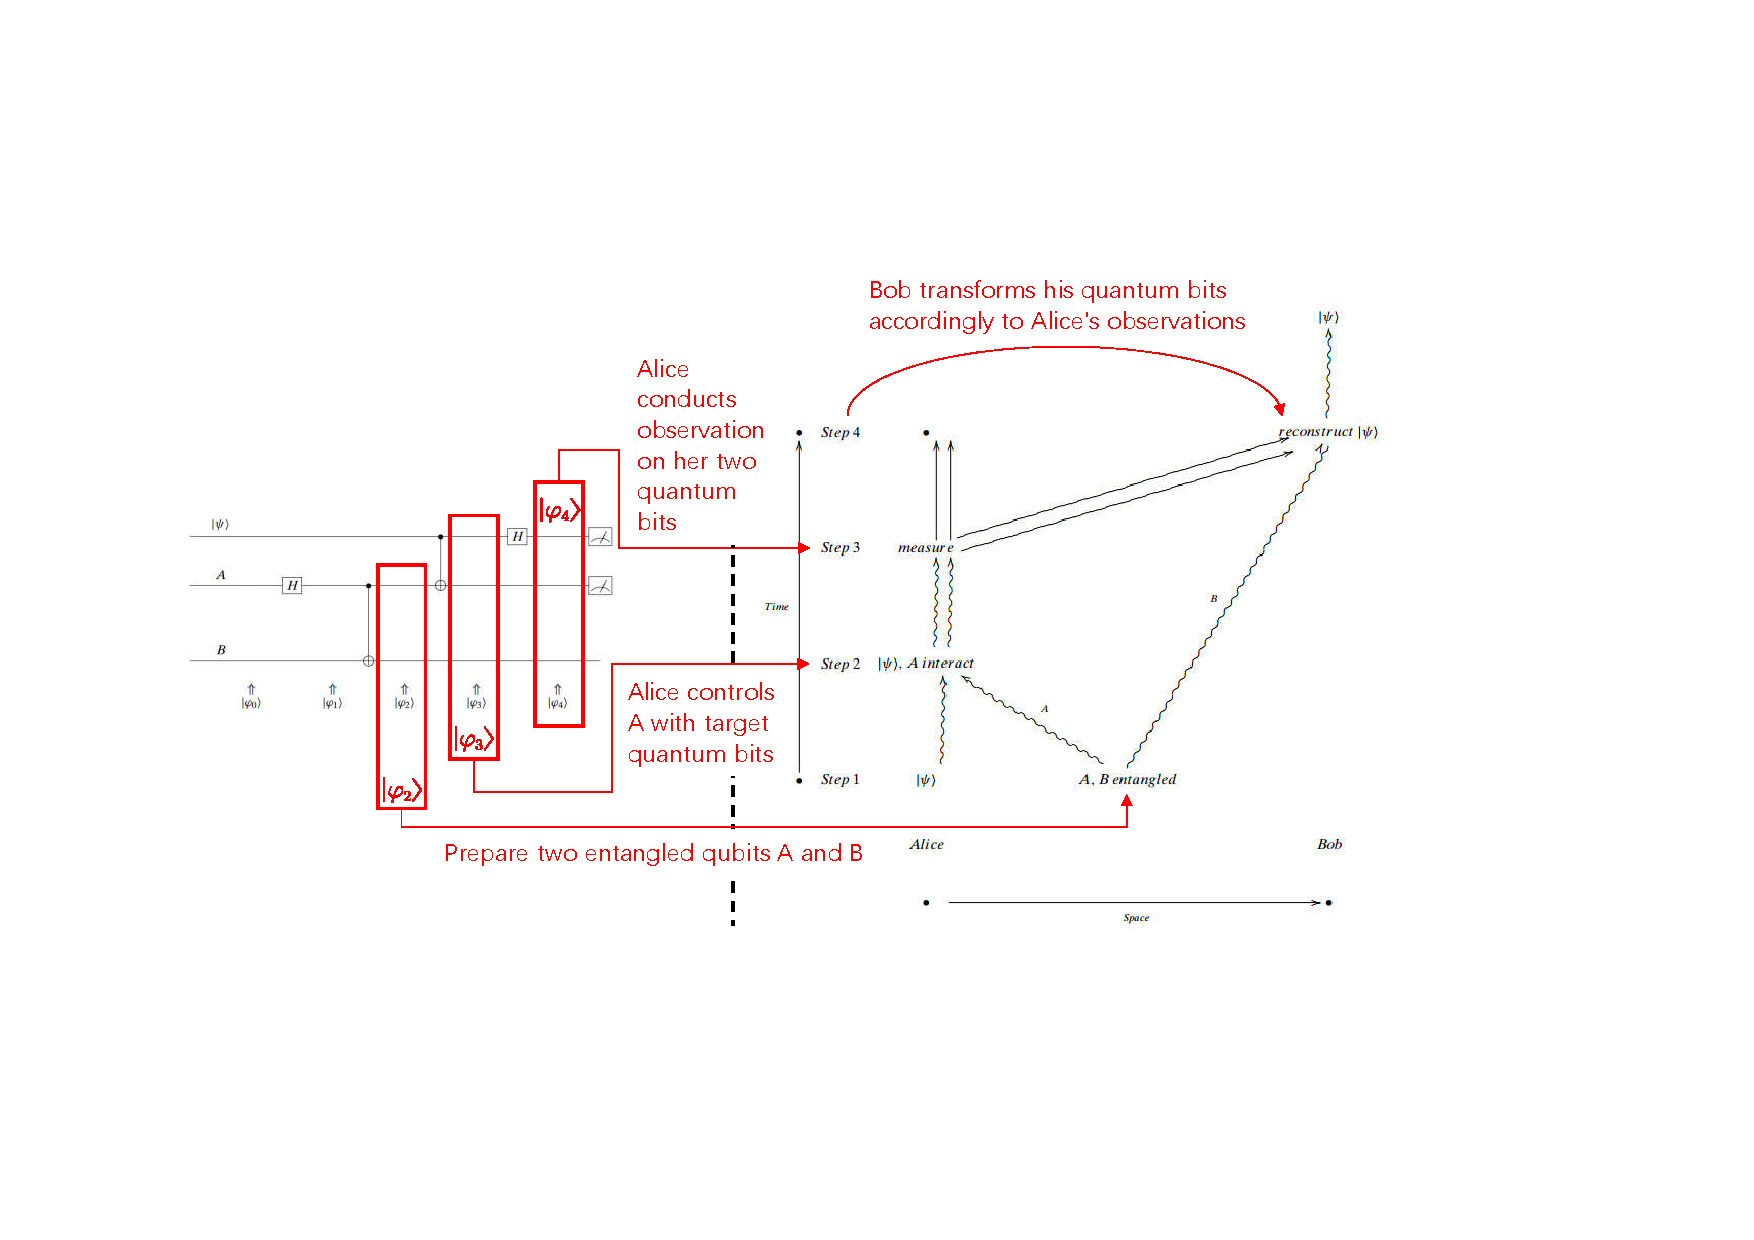
\includegraphics[width=0.9\textwidth]{qt-framework}
	\caption{The framework of quantum teleportation protocol.}
	\label{fig:qt-framework}
\end{figure}



\curinstructor{Chao Liang}

\ifx\flag\undefined
	\end{document}
\else